% CatSight AI thesis (revised edition). Build with ./build.sh (XeLaTeX + BibTeX).
\documentclass[12pt,a4paper,oneside]{report}

% --- Page, fonts, spacing --------------------------------------------------------------
\usepackage[margin=1in]{geometry}
\usepackage{fontspec}
\usepackage{unicode-math}
\setmainfont{Times New Roman}
\setmathfont{STIX Two Math}
\setmonofont{Menlo}[Scale=0.82]
\usepackage{setspace}
\doublespacing
\usepackage{microtype}
\setlength{\emergencystretch}{3em}
\usepackage[english]{babel}
\usepackage{csquotes}
\setlength{\parindent}{0.5in}

% --- Headings: bold, left-aligned, as in the defended paper -----------------------------
\usepackage{titlesec}
\titleformat{\chapter}[block]{\normalfont\large\bfseries}{Chapter \thechapter}{0.5em}{}
\titlespacing*{\chapter}{0pt}{0pt}{12pt}
\titleformat{\section}{\normalfont\normalsize\bfseries}{\thesection}{0.6em}{}
\titleformat{\subsection}{\normalfont\normalsize\bfseries}{\thesubsection}{0.6em}{}
\titleformat{\subsubsection}{\normalfont\normalsize\bfseries\itshape}{\thesubsubsection}{0.6em}{}
\titlespacing*{\section}{0pt}{12pt}{0pt}
\titlespacing*{\subsection}{0pt}{12pt}{0pt}
\titlespacing*{\subsubsection}{0pt}{12pt}{0pt}
\setcounter{secnumdepth}{3}
\setcounter{tocdepth}{2}

% --- Math, tables, lists ------------------------------------------------------------------
\usepackage{amsmath}
\usepackage{array,booktabs,longtable,tabularx,multirow,makecell}
\renewcommand{\arraystretch}{1.15}
\usepackage{enumitem}
\setlist{nosep,leftmargin=*,labelindent=0.5in}
\usepackage{etoolbox}

% --- Figures: one width rule for every figure (revision 2) -------------------------------
\usepackage{graphicx}
\usepackage{float}
\usepackage{placeins}
\usepackage{xcolor}
\definecolor{maroon}{HTML}{9C162D}
\definecolor{ink}{HTML}{1F1A1B}
\definecolor{soft}{HTML}{F6F2EE}
\definecolor{line}{HTML}{BDB3AE}
\definecolor{gold}{HTML}{C9A227}
\usepackage{tikz}
\usetikzlibrary{arrows.meta,positioning,fit,backgrounds,calc,shapes.geometric,shapes.multipart}
\usepackage{pgfplots}
\pgfplotsset{compat=1.18}
\tikzset{
  every picture/.style={font=\small\linespread{1}\selectfont, line width=0.6pt},
  every node/.append style={execute at begin node={\hyphenpenalty=10000\exhyphenpenalty=10000}},
  box/.style={draw=ink, rounded corners=2pt, fill=white, align=center, inner sep=5pt, text width=#1},
  box/.default=2.6cm,
  accent/.style={box=#1, draw=maroon, fill=maroon!6},
  accent/.default=2.6cm,
  muted/.style={box=#1, draw=line, fill=soft},
  muted/.default=2.6cm,
  arrow/.style={-{Stealth[length=2.2mm]}, draw=ink},
  dashedarrow/.style={arrow, dashed},
  note/.style={font=\footnotesize, text=ink!80, align=center},
  group/.style={draw=line, dashed, rounded corners=4pt, inner sep=8pt},
}

\usepackage[font={normalsize,singlespacing}, labelfont=bf, textfont=it, labelsep=period,
            justification=centering, skip=6pt]{caption}
\captionsetup[table]{position=top}
% A screenshot at full text width with a hairline frame, so white UI edges don't vanish on paper
\newcommand{\screenshot}[3][\linewidth]{%
  \begin{figure}[htbp]
    \centering
    {\setlength{\fboxsep}{0pt}\setlength{\fboxrule}{0.4pt}\color{line}%
     \fbox{\includegraphics[width=\dimexpr#1-0.8pt\relax]{screenshots/#2}}}
    \caption{#3}\label{fig:#2}
  \end{figure}}

% --- Algorithms (revisions 13 and 18) ----------------------------------------------------
\usepackage[ruled,vlined,linesnumbered]{algorithm2e}
\SetAlFnt{\small}
\SetAlCapFnt{\normalsize}
\SetAlCapNameFnt{\normalsize\itshape}
\SetKwInput{KwIn}{Input}
\SetKwInput{KwOut}{Output}
\SetKwProg{Fn}{function}{}{}
\SetKwComment{tcp}{$\triangleright$\ }{}
\newcommand{\algcommentfont}[1]{\footnotesize\itshape\textcolor{ink!70}{#1}}
\SetCommentSty{algcommentfont}
\AtBeginEnvironment{algorithm}{\setstretch{1.1}}
\AtBeginEnvironment{tabular}{\setstretch{1.0}}
\AtBeginEnvironment{tabularx}{\setstretch{1.0}}
\AtBeginEnvironment{longtable}{\setstretch{1.0}}

% --- Citations: APA-like author-year (natbib + apalike) ----------------------------------
\usepackage[authoryear,round]{natbib}
\setlength{\bibsep}{6pt}
\setlength{\bibhang}{0.5in}

% --- Links and lists of floats -----------------------------------------------------------
\usepackage{tocloft}
\renewcommand{\cftchapfont}{\bfseries}
\renewcommand{\cftchappagefont}{\bfseries}
\renewcommand{\cftchapleader}{\cftdotfill{\cftdotsep}}
\renewcommand{\cftchappresnum}{Chapter~}
\setlength{\cftchapnumwidth}{5.4em}
\usepackage{xurl}
\usepackage[hidelinks,bookmarksnumbered]{hyperref}

% Data the panel's revisions still need from the proponents: shown in the PDF so none is missed
\newcommand{\TODO}[1]{\textcolor{maroon}{\textbf{[TODO: #1]}}}
\newcommand{\code}[1]{\texttt{#1}}
\newcommand{\cs}{CatSight AI}

\begin{document}

\pagenumbering{roman}
\begin{titlepage}
  \centering
  \singlespacing
  {\bfseries CatSight AI: Enhancing Document Search Accuracy and User Interaction through OCR,\\[4pt]
   Vector Similarity Search, and LLM-Based Chat Interfaces\par}
  \vspace{2.2cm}
  {\bfseries A Thesis Project\par}
  \vspace{1cm}
  {\bfseries Submitted to\par}
  \vspace{1cm}
  {\bfseries The Faculty of the Department of Computer Science\\[4pt]
   Mindanao State University -- Iligan Institute of Technology\\[4pt]
   In Fulfillment of the Requirements in CSC198 -- Research Method\par}
  \vspace{2cm}
  Arellano, Carlo P.\\[4pt]
  Carnaje, Michael James M.\\[4pt]
  Lavesores, Fulgent Kvasir E.\\[4pt]
  {\bfseries Proponents\par}
  \vspace{2.5cm}
  Professor Dante D. Dinawanao\\[4pt]
  {\bfseries Adviser\par}
  \vfill
  Revised edition, October 2026
\end{titlepage}

\chapter*{Revision Summary}
\addcontentsline{toc}{chapter}{Revision Summary}

\begingroup
\small
\setstretch{1.0}
\begin{longtable}{@{}p{1.6cm}p{8.4cm}p{4.4cm}@{}}
  \toprule
  \textbf{Revision No.} & \textbf{Details} & \textbf{Section / Page No.} \\
  \midrule
  \endhead
  1 & Missing Theoretical Framework & Methodology, Page 34 \\
  2 & Be proper and consistent with the figure sizes, and make it clearer & Methodology Page 40 \\
  3 & Add Design and Implementation Issue & Methodology, Page 34 \\
  4 & Proper spacing & Methodology. Pag 44 \\
  5 & Missing Summarization Figure flow & Methodology, Page 44 \\
  6 & Use Rouge, Bleu, Bertscore for Summarization Metrics & Methodology \\
  7 & Mention the figures that are shown & Methodology \\
  8 & Use LaTex Equation & Methodology \\
  10 & Provide cosine similarity score equations &  \\
  11 & Explain Token and Cosine Similarity Score &  \\
  12 & Discuss the map reduce in the paper &  \\
  13 & Write algorithm for generate summary &  \\
  14 & Define hallucination in LLM and its basis &  \\
  15 & Explain zero-shot method &  \\
  16 & Specific objective be more concise & Specific Objective Page 4 \\
  17 & Show a architecture diagram to show the interactions of each component & 3.2 methodology. Page 37 \\
  18 & Express the diagrams in algorithm instead of flow charts &  \\
  \bottomrule
\end{longtable}
\endgroup
\clearpage

\chapter*{Abstract}
\addcontentsline{toc}{chapter}{Abstract}

The CatSight AI system addresses the limitations of MSU-IIT’s keyword-based document search by leveraging a unified pipeline of OCR, vector embeddings, and an LLM-driven conversational interface. The architecture follows a retrieval-augmented generation (RAG) framework: documents (scanned or digital) are processed via OCR (ensuring text extraction from scanned or image-based documents), segmented into chunks, embedded into vector representations stored in a vector database, and then retrieved to support LLM response generation. This integration enables users to issue intuitive natural-language queries and receive contextually relevant answers through a chat-based interface.

In evaluations against the legacy system, CatSight AI achieved higher retrieval accuracy, semantic relevance, and efficiency. The hybrid approach substantially improves semantic understanding, capturing paraphrases and synonyms (for example, equating “academic calendar” with “term schedule”) that the keyword system misses, and retrieves more relevant results than keyword-only search. User testing confirmed a marked usability gain: CatSight’s System Usability Scale score averaged 77.17\%, versus only 50.33\% for the existing system. Overall, these results indicate that CatSight AI outperforms traditional methods in search accuracy and user experience, offering a more accurate, intelligent, and efficient document retrieval solution.

\vspace{1em}
\noindent\textbf{Keywords:} \emph{Document Retrieval System, Optical Character Recognition (OCR), Vector-Based Similarity Search, Large Language Model (LLM), Semantic Search}
\clearpage


\begin{singlespace}
\tableofcontents
\clearpage
\listoffigures
\clearpage
\listoftables

\end{singlespace}
\clearpage

\pagenumbering{arabic}
\chapter{Research Description}\label{ch:description}

In today’s era of digital transformation, organizations generate and store an unprecedented volume of documents daily. This exponential growth in document storage has created a pressing demand for efficient document retrieval systems (DRS) to access, manage, and leverage information effectively. A document retrieval system is a specialized application of information retrieval (IR) designed to locate relevant documents within vast repositories based on user queries. By enabling quick and accurate access to information, DRS plays a pivotal role in knowledge management, informed decision-making, and productivity enhancement across diverse domains, including education, business, healthcare, and research (Blair, n.d.; Macdonald \& Tait, 2020).

At its core, document retrieval addresses the challenge of identifying stored documents that contain pertinent information. The primary objective is to distinguish between relevant and non-relevant documents for a user’s specific query. Modern DRS employs various techniques to achieve this, ranging from traditional keyword-based methods to advanced machine learning approaches. Keyword-based retrieval is a foundational technique that matches user queries to specific keywords within documents. While it is straightforward and easy to implement, its reliance on exact matches can limit its ability to capture the broader context of queries (Blair, n.d.). Boolean retrieval, an early and widely used approach, utilizes logical operators like AND, OR, and NOT to narrow down search results based on exact keyword matches. Though simple, it often lacks the flexibility to handle nuanced user queries (Macdonald \& Tait, 2020). The Vector Space Model (VSM) improves on this by representing documents and queries as vectors in a multi-dimensional space, with relevance determined by the cosine similarity between these vectors, enabling more precise ranking of results compared to Boolean methods (Blair, n.d.). Latent Semantic Analysis (LSA) takes this further by uncovering hidden relationships between terms in a document collection through term-document matrix analysis, thereby enhancing retrieval accuracy by capturing the semantic meaning of words rather than relying solely on exact matches (Macdonald \& Tait, 2020). Machine learning-based retrieval techniques, such as support vector machines (SVMs), random forests, and deep learning models, dynamically adapt to user behavior and context, significantly enhancing retrieval accuracy (Blair, 1984). Neural information retrieval systems, leveraging advanced deep learning architectures like recurrent neural networks (RNNs) and transformers, model complex language patterns and contextual nuances in documents, offering even greater precision and relevance in search results (Macdonald \& Tait, 2020).

A notable advancement in modern DRS is the integration of Retrieval-Augmented Generation (RAG) frameworks. RAG combines document retrieval with generative AI models to provide highly contextual and human-like responses. This approach retrieves relevant documents from the repository and feeds them into generative models, like GPT, which synthesize coherent and informative answers to user queries. The RAG framework not only enhances the retrieval process but also bridges the gap between static document retrieval and dynamic information synthesis, making it a revolutionary tool in data-driven environments (Macdonald \& Tait, 2020).

This research aims to explore the evolving landscape of document retrieval systems, emphasizing their significance in transforming data into actionable knowledge. By analyzing advanced retrieval techniques and highlighting the role of RAG, this study underscores the pivotal role of DRS in fostering innovation and informed decision-making in the digital age.

\section{Background of the Study}

Effective management and access to extensive information repositories are crucial for institutions that maintain vast collections of documents. Document Retrieval Systems (DRS) are essential tools that enable users to efficiently locate specific documents. This study focuses on the Mindanao State University – Iligan Institute of Technology (MSU-IIT), which has its own repositories for Special Orders, Memorandums, and other important records. MSU-IIT maintains two primary repositories:

\begin{itemize}
  \item \textbf{Board of Regents (BOR) Resolutions Archive:} This repository contains BOR resolutions of the MSU System. (Mindanao State University - Iligan Institute of Technology, n.d.-a)
  \item \textbf{IIT Docs:} This repository houses Special Orders, Memorandum Orders, and other issuances of MSU-IIT. (Mindanao State University - Iligan Institute of Technology, n.d.-b)
\end{itemize}

Both repositories utilize keyword-based document search mechanisms. IIT Docs, for instance, is built on top of Google Drive and leverages its search capabilities.

While functional, the current keyword-based approach presents several challenges that limit its effectiveness. Keyword searches often fail to account for the context or semantics of user queries, leading to inaccurate or irrelevant search results. Users frequently encounter difficulties in locating exact documents based on their information needs, particularly when dealing with large or complex datasets. This issue is particularly pronounced at MSU-IIT, where reliance on traditional keyword-based models highlights significant gaps in accuracy and efficiency.

In the advent of large language models, the MSU-IIT repository can benefit from enhanced search capabilities that understand the context and semantics of user queries, potentially improving the precision and efficiency of document retrieval.

The current system's gap lies in its inability to comprehend the semantic nuances of user queries, limiting its effectiveness in handling large or complex datasets. As a result, the system is held back in providing a streamlined and user-friendly retrieval process. This inefficiency hinders the institution's ability to fully leverage its vast repository of documents, affecting productivity and decision-making processes.

The study was conducted to address these limitations and explore potential solutions to enhance document retrieval at MSU-IIT. By investigating advanced approaches such as content-based retrieval systems, which will utilize technologies like Optical Character Recognition (OCR), vector embeddings, and Large Language Model (LLM)-powered conversational interfaces, the research will aim to improve search accuracy, user experience, and overall system efficiency. This initiative will seek to bridge the gap between traditional methods and modern technological capabilities, ensuring that MSU-IIT can effectively meet the demands of its users and maintain operational excellence.

\section{Statement of the Problem}

Traditional keyword-based document retrieval systems face global challenges in providing accurate and relevant results due to their lack of contextual and semantic understanding. This often leads to inefficient search experiences for users worldwide. At MSU-IIT, students, faculty, and staff experience similar issues when retrieving institutional documents. The current system’s reliance on exact keyword matches limits access to important information. A more advanced, context-aware solution is needed to address these limitations and position MSU-IIT as a model for modern document retrieval.

\section{Research Objective}

The following are the general and specific objects:

\subsection{General Objective}

To develop and evaluate a content-based document retrieval system that integrates Optical Character Recognition (OCR), vector embeddings, and Large Language Model (LLM)-powered conversational interaction.

\subsection{Specific Objective}\label{sec:objectives}

\begin{enumerate}
  \item To collect and annotate representative documents from MSU-IIT’s institutional repositories, specifically IIT Docs and BOR Resolutions.
  \item To design a content-based document retrieval system architecture integrating OCR for scanned PDFs, vector embeddings for semantic search, and LLMs for conversational queries.
  \item To implement the system’s key components: OCR processing, semantic search using vector similarity, and an LLM-based chat interface.
  \item To evaluate the system’s performance in terms of accuracy, user experience, and retrieval speed.
  \item To analyze evaluation results to validate system effectiveness and recommend future enhancements.
\end{enumerate}

\section{Scope and Limitations of the Research}\label{sec:scope}

This study focuses on enhancing the Document Retrieval System (DRS) at Mindanao State University - Iligan Institute of Technology (MSU-IIT). The research will involve a sample of 50 PDF documents and will be conducted from January 2025 to April 2025, with participants including MSU-IIT students, faculty, and staff. A notable limitation of the current system is its inability to analyze images and tables within documents, restricting its effectiveness in processing non-textual data. This constraint may impact the retrieval accuracy for documents where critical information is presented in these formats. By acknowledging this limitation, the study aims to provide a clear understanding of the system's current capabilities and identify areas for improvement to effectively meet the institution's document retrieval needs.

\section{Significance of the Study}

This study holds significant value not only for MSU-IIT students, staff, and faculty but also for other institutions and entities that require efficient document storage and retrieval systems. It aims to enhance the overall efficiency and effectiveness of managing and accessing documents within an organization.

\chapter{Review of Related Literature}\label{ch:rrl}

This chapter explores the foundational principles and advancements in document retrieval systems. It examines the traditional title and keyword-based search methods alongside the more sophisticated content-based approaches. A comparative analysis is provided, highlighting the strengths, limitations, and applications of these systems in addressing the evolving demands of users. By delving into the role of OCR, vector embeddings, and LLMs, this review sets the stage for evaluating how content-based systems redefine document retrieval processes in terms of accuracy, efficiency, and user satisfaction.

\section{Document and Information Retrieval Systems}

In the modern era of digital transformation, organizations generate and store vast volumes of documents daily. This exponential growth in document storage has created an urgent need for efficient document retrieval systems (DRS) to access, manage, and utilize information effectively. A document retrieval system is a specialized application of information retrieval (IR) focused on locating relevant documents from a repository based on user queries. It plays a crucial role in knowledge management, decision-making, and enhancing productivity across various domains, including education, business, healthcare, and research.

Document retrieval is the problem of finding stored documents that contain useful information. According to Blaire et al.., (n.d.), There exist a set of documents on a range of topics, written by different authors, at different times, and at varying levels of depth, detail, clarity, and precision, and a set of individuals who, at different times and for different reasons, search for recorded information that may be contained in some of the documents in this set. In each instance in which an individual seeks information, he or she will find some documents of Ihe set useful and other documents not useful; the documents found useful are, we say. relevant; the others, not relevant. In order for a person to find all and only the relevant items in a collection of stored documents; one answer is automatic full-text retrieval, which on its surface is disarmingly simple: Store the full text of all documents in the collection on a computer so that every character of every word in every sentence of every document can be located by the machine. Then, when a person wants information from that stored collection, the computer is instructed to search for all documents containing certain specified words and word combinations, which the user has specified (MacDonald \& Tonelleto, 2020).

\subsection{COIL: Revisit Exact Lexical Match in Information Retrieval with Contextualized Inverted List}

In the realm of information retrieval, traditional systems like BM25 have long relied on exact lexical matches, efficiently utilizing inverted list indexes to retrieve documents. However, these systems often struggle with vocabulary mismatches and fail to capture the semantic nuances of language. Conversely, recent neural information retrieval (IR) models emphasize soft semantic matching across all query-document terms, enhancing semantic understanding but at the cost of computational efficiency. Addressing this dichotomy, Gao, Dai, and Callan (2021) introduced the Contextualized Inverted List (COIL) architecture, which aims to integrate the efficiency of exact lexical matching with the semantic depth provided by deep language models.

COIL innovatively stores contextualized token representations within inverted lists, enabling the system to perform exact matches based on the contextual meaning of terms rather than solely on their surface forms. This approach allows COIL to leverage the rich semantic information captured by deep language models while maintaining the retrieval speed characteristic of traditional inverted index structures. By focusing on overlapping query-document tokens' contextualized representations, COIL effectively bridges the gap between lexical and semantic matching. Empirical evaluations demonstrate that COIL outperforms both classical lexical retrievers and state-of-the-art deep language model retrievers, achieving superior retrieval effectiveness with comparable or reduced latency. This performance underscores COIL's capability to deliver precise and contextually relevant results without compromising on efficiency.

The introduction of COIL represents a significant advancement in document and information retrieval systems. By harmonizing the strengths of exact lexical matching and semantic understanding, COIL addresses longstanding challenges such as vocabulary mismatch and semantic ambiguity. Its design offers a practical solution for developing retrieval systems that are both effective and efficient, making it a valuable reference for researchers and practitioners aiming to enhance retrieval performance in various applications.

\section{Embeddings in Document Retrieval}

In the realm of information retrieval, traditional methods have predominantly relied on keyword matching, which often falls short in capturing the nuanced meanings inherent in human language. This limitation has spurred the development of embedding techniques that represent words, sentences, and documents as vectors in high-dimensional space, effectively encoding semantic relationships. By transcending the constraints of exact keyword matches, embeddings facilitate a more profound understanding of context and intent, thereby significantly enhancing the precision and recall of document retrieval systems.

Embeddings represent words, phrases, or documents as vectors in a continuous vector space, enabling systems to measure semantic similarity between textual elements. This representation facilitates the retrieval of documents that are contextually relevant, even when there is no exact keyword match. For instance, embedding-based retrieval systems can recognize that the terms "car" and "automobile" are semantically related, retrieving pertinent documents regardless of the specific term used in the query (Mikolov et al., 2013; Devlin et al., 2019).

Mikolov et al. (2013) introduced word embeddings through the word2vec model, which revolutionized natural language understanding by encoding semantic relationships in vector space. Later advancements, such as BERT (Devlin et al., 2019), extended this concept by producing contextualized embeddings that capture meanings based on surrounding text. These advancements have made embedding-based approaches foundational in modern information retrieval, including models like RepBERT (Zhan et al., 2020), which demonstrated the effectiveness of embeddings in document ranking tasks.

The integration of embeddings into retrieval systems has led to significant improvements in performance. For instance, Huang et al. (2020) implemented embedding-based retrieval in Facebook Search, resulting in enhanced search relevance and user satisfaction. Similarly, Zhan et al. (2020) introduced RepBERT, a model that represents documents and queries with fixed-length contextualized embeddings, achieving state-of-the-art results in initial retrieval tasks.

The adoption of embedding techniques marks a pivotal advancement in document retrieval, enabling systems to move beyond simple keyword matching to a more nuanced understanding of language. This evolution has significantly improved the precision and recall of retrieval systems, aligning them more closely with human language understanding and enhancing the overall user experience.

\subsection{Embedding-based Retrieval in Facebook Search}

Facebook Search is a feature that enables users to locate content within the Facebook platform, including profiles, pages, groups, posts, and other entities. Unlike traditional web search engines, Facebook Search must consider the unique context of each user, such as their social connections and personal interactions, to deliver relevant results. This personalized approach leverages the user's social graph to enhance the search experience (Huang et al., 2020).

According to Huang et al., (2020), “historically, Facebook Search relied on Boolean matching models, which focus on exact keyword matches. However, this method often failed to capture the nuanced meanings and contextual relevance of queries, leading to less satisfactory user experiences”. To address these limitations, Facebook implemented Embedding-Based Retrieval (EBR) techniques. EBR represents queries and documents as vectors in a continuous vector space, allowing the system to measure semantic similarities between them. This approach enables the retrieval of contextually relevant information, even when there is no exact keyword match.

The adoption of EBR in Facebook Search has significantly improved the relevance of search results and user satisfaction. By understanding the semantic relationships between queries and documents, the system can provide more accurate and personalized results. For instance, if a user searches for "apple," the system can discern whether the user is interested in the fruit or the technology company based on contextual cues, thereby delivering appropriate results. This advancement aligns with the findings of Huang et al. (2020), who reported significant metric gains in online A/B experiments after implementing EBR in Facebook Search.

In summary, the integration of embedding-based retrieval techniques into Facebook Search has transformed the platform's ability to deliver semantically relevant and personalized search results, thereby enhancing overall user satisfaction.

\subsection{RepBERT: Contextualized Text Embeddings for First-Stage Retrieval}

In the realm of information retrieval, traditional first-stage retrieval methods have predominantly relied on exact term matching techniques, such as bag-of-words models. While these methods are computationally efficient, they often fail to capture the semantic nuances of language, leading to suboptimal retrieval performance. To address these limitations, Zhan et al. (2020) introduced RepBERT, a model that leverages fixed-length contextualized embeddings to represent both queries and documents. By computing the inner products of these embeddings as relevance scores, RepBERT effectively captures semantic relationships, thereby enhancing retrieval accuracy.

According to Zhan, J., et al. (2020), ‘traditional exact term matching methods, such as BM25, depend on the presence of identical terms in both queries and documents. This reliance can result in missed relevant documents that use synonymous or semantically related terms’. RepBERT addresses this issue by encoding the contextual meaning of text into dense vectors, allowing for the recognition of semantic similarities even in the absence of exact term matches. For example, RepBERT can identify that "car" and "automobile" refer to the same concept, thus retrieving pertinent documents regardless of the specific term used in the query.

In the study by Zhan, J., Mao, J., Liu, Y., Zhang, M., \& Ma, S. (2020), RepBERT represents documents and queries with fixed-length contextualized embeddings, using their inner products as relevance scores. This method achieves state-of-the-art results in initial retrieval tasks, balancing effectiveness and efficiency.

\subsection{CLEAR}

In information retrieval, traditional lexical models like BM25 rely on exact term matching, which can overlook semantic nuances and lead to issues such as vocabulary mismatch. To address these limitations, Gao et al. (2020) introduced the Complement Lexical Retrieval Model with Semantic Residual Embeddings (CLEAR). CLEAR enhances retrieval performance by integrating semantic matching signals from neural embeddings with traditional lexical retrieval methods.

The information regarding the Complement Lexical Retrieval Model with Semantic Residual Embeddings (CLEAR) is sourced from the study by Gao et al. (2020). In their research, they introduce CLEAR, a retrieval model that enhances traditional lexical retrieval methods like BM25 by incorporating semantic matching signals derived from neural embeddings. This integration is achieved through a novel residual-based embedding learning method, which trains the neural embeddings to capture language structures and semantics that lexical retrieval models may overlook. Empirical evaluations conducted in the study demonstrate that CLEAR outperforms state-of-the-art retrieval models, significantly improving both the accuracy and efficiency of reranking pipelines.

By combining the strengths of lexical and semantic retrieval methods, CLEAR offers a more robust solution to the challenges of information retrieval, effectively bridging the gap between exact term matching and semantic understanding.

\subsection{Automatic Document Screening of Medical Literature Using Word and Text Embeddings in an Active Learning Setting}

In Evidence-Based Medicine (EBM), document screening is essential for providing scientific evidence to support medical decisions. However, the exponential growth of medical literature has made this task increasingly time-consuming and labor-intensive for physicians. To address this challenge, Carvallo et al. (2020) investigated the use of word and text embeddings within an active learning framework to semi-automate the document screening process.

Implementing semi-automated screening methods can significantly alleviate the burden on healthcare professionals, allowing them to focus more on patient care and critical decision-making. By efficiently identifying relevant studies, these methods enhance the quality and timeliness of medical evidence synthesis, ultimately leading to improved patient outcomes. Moreover, the integration of advanced natural language processing techniques, such as word and text embeddings, enables the system to capture complex semantic relationships within the literature, further improving the accuracy of the screening process.

The approach proposed by Carvallo et al. (2020) has practical applications in various medical fields, including the development of clinical guidelines, systematic reviews, and meta-analyses. By reducing the manual effort required for literature screening, it facilitates the timely incorporation of the latest research findings into clinical practice, thereby supporting the continuous advancement of healthcare quality.

\section{Information Extraction and Retrieval from PDF Documents}

The Portable Document Format (PDF) is a widely adopted standard for disseminating digital documents across various domains, including academia, business, and government. Its design ensures consistent presentation across different platforms and devices, encapsulating text, images, and complex layouts. However, this fixed-layout nature poses challenges for information extraction and retrieval, as the format prioritizes visual fidelity over structural representation.

The significance of information extraction and retrieval from PDF documents lies in its ability to unlock valuable data embedded within these widely used files. By facilitating access to information that might otherwise remain obscured, effective PDF data extraction enhances data accessibility (Livathinos et al., 2021). Transforming unstructured PDF content into structured data further improves search capabilities, allowing users to efficiently locate specific information. This process also supports better knowledge management within organizations, enabling them to manage and utilize extracted information for informed decision-making and streamlined workflows (Clark et al., n.d).

The evolution of information extraction and retrieval from PDF documents reflects significant technological advancements. Initially, information was manually extracted from PDFs, a labor-intensive and error-prone process (Clark et al., n.d.). This was followed by the introduction of rule-based systems, which used predefined rules and templates to identify and extract data. While these systems provided some automation, they struggled with diverse document layouts and lacked scalability. The emergence of machine learning marked a transformative phase, with models capable of learning from annotated data, thereby improving extraction accuracy and adaptability to various document structures (Palm et al., 2017). More recently, deep learning techniques have revolutionized the field by leveraging neural networks to capture complex patterns and relationships within documents. These advancements have significantly enhanced the performance of information extraction systems, enabling more effective processing of PDF content (Gupta et al., 2018).

\subsection{BEIR}

The Benchmarking Information Retrieval (BEIR) dataset is a comprehensive benchmark designed to evaluate the zero-shot performance of information retrieval models across a diverse array of tasks and domains. Introduced by Thakur et al. (2021), BEIR encompasses 18 publicly available datasets, each representing unique retrieval challenges, including fact-checking, question answering, and biomedical information retrieval. This diversity enables researchers to systematically assess how well retrieval models generalize to new, unseen scenarios without domain-specific training.

A key feature of BEIR is its facilitation of zero-shot evaluation, where models are tested on datasets they were not specifically trained on. This approach provides critical insights into a model's out-of-distribution generalization capabilities, reflecting its robustness and applicability in real-world situations where annotated data may be scarce. By offering a standardized framework, BEIR allows for consistent and fair comparisons among various retrieval systems, including lexical, sparse, dense, late-interaction, and re-ranking architectures.

The significance of BEIR lies in its role as a unifying benchmark that addresses the limitations of previous evaluations, which often focused on narrow or homogeneous settings. By encompassing a wide range of tasks and domains, BEIR challenges models to perform well across different types of retrieval scenarios, thereby promoting the development of more robust and versatile information retrieval systems. The benchmark's comprehensive nature encourages the advancement of models capable of effective zero-shot retrieval, ultimately contributing to more adaptable and efficient information retrieval technologies.

\subsection{Declarative Experimentation in Information Retrieval using PyTerrier}

In the field of information retrieval (IR), constructing and evaluating complex retrieval pipelines can be a challenging endeavor, often requiring intricate coding and deep system knowledge. To address these challenges, Macdonald and Tonellotto (2020) introduced PyTerrier, a Python-based framework that facilitates declarative experimentation in IR. PyTerrier enables researchers and practitioners to express retrieval pipelines in a manner that closely aligns with their conceptual design, thereby simplifying the experimentation process.

Prior to the development of PyTerrier, the IR community lacked a formalism that allowed for the expressive representation of complex retrieval pipelines in high-level programming languages. Existing tools often required extensive coding and were not conducive to rapid experimentation or reproducibility. Macdonald and Tonellotto identified this gap and proposed PyTerrier as a solution to enable declarative experimentation, thereby addressing the need for a more efficient and collaborative approach to IR research.

The significance of PyTerrier lies in its ability to streamline the development and evaluation of retrieval systems. By allowing users to construct retrieval pipelines declaratively, PyTerrier reduces the complexity associated with traditional procedural programming approaches. This declarative paradigm enhances reproducibility in IR research, as experiments can be easily shared and replicated. Moreover, PyTerrier's integration with existing IR platforms, such as Anserini and Terrier, enables seamless execution and evaluation of retrieval pipelines, fostering collaboration and innovation within the research community.

\section{Large Language Models (LLMs) in Information Retrieval}

Large Language Models (LLMs) have significantly advanced Information Retrieval (IR), especially in handling complex document formats like PDFs. PDFs are widely used in academia, business, and government because of their consistent visual presentation across platforms, but their fixed layout makes extracting and retrieving information challenging. Earlier methods such as manual extraction, rule-based systems, and early machine learning models often struggled with the diversity and complexity of PDF structures. The introduction of deep learning and neural networks improved this process by allowing systems to recognize complex patterns and better understand document structures.

LLMs like GPT models have further transformed IR by enabling a deeper understanding of natural language and user intent. These models can interpret nuanced queries, retrieve relevant information without relying on exact keyword matches, and support conversational, personalized, and cross-language search. This enhances user experience and makes information more accessible. As LLMs continue to improve, their integration into IR systems promises to make data from documents like PDFs more searchable, accessible, and useful for knowledge management across many fields.

\subsection{Large Language Models for Information Retrieval: A Survey}

Large Language Models (LLMs) have significantly enhanced Information Retrieval (IR) by improving key components such as query rewriting, retrieval, reranking, and reading (Zhu et al., 2023). LLMs excel at interpreting complex user queries by capturing semantic meaning beyond keyword matching, leading to more accurate and relevant document retrieval. They generate contextual embeddings that align with user intent and can rerank documents based on content relevance. Additionally, LLMs synthesize information from multiple sources to provide coherent and informative responses.

The integration of LLMs into IR systems supports natural language interactions, personalized search, multilingual retrieval, and domain-specific applications in fields like healthcare and law (Zhu et al., 2023). However, challenges remain, including the need for large training datasets, limited interpretability, and high computational requirements. Addressing these issues is essential for maximizing the potential of LLMs in improving search relevance and information accessibility.

\subsection{Fine-Tuning LLaMA for Multi-Stage Text Retrieval}

Text retrieval is essential for tasks such as web search, open-domain question answering, and fact verification, and it plays a key role in enhancing large language models (LLMs) within retrieval-augmented generation (RAG) pipelines. This integration helps reduce hallucinations and allows LLMs to access external knowledge (Ma et al., 2024). Recent LLMs like GPT-4 and LLaMA have shown remarkable performance across various NLP tasks, with new methods such as RankGPT, LRL, and PRP using prompting techniques to perform zero-shot listwise or pairwise ranking as generative tasks (Ma et al., 2024).

Ma et al. (2024) explore fine-tuning the LLaMA model for multi-stage text retrieval, which involves an initial coarse retrieval phase followed by refined reranking steps. This approach leverages LLaMA’s advanced language understanding to improve retrieval accuracy, particularly in tasks requiring deep contextual comprehension and precise ranking.

\section{AI-Powered Prompt-Based Information Extraction}

AI-powered prompt-based information extraction enables efficient retrieval of structured data from unstructured text by leveraging Large Language Models (LLMs) with well-crafted prompts (Xu et al., 2023; Çöplü et al., 2024). Unlike rule-based systems, prompt-based methods are flexible and easily adaptable to new tasks by simply modifying the input prompts, reducing development time and effort (Xu et al., 2024; Do et al., 2024). This approach is widely used in fields such as law, healthcare, and business intelligence to extract relevant information from complex documents (Xu et al., 2023; Wei et al., 2023). However, its effectiveness relies heavily on prompt design, as poorly constructed prompts can lead to inaccurate results (Çöplü et al., 2024; Do et al., 2024).

\subsection{Prompt-Time Symbolic Knowledge Capture with Large Language Models}

In their 2024 study, Çöplü et al. address a critical challenge in the deployment of Large Language Models (LLMs) for personalized applications: the models' inherent inability to capture and utilize user-specific knowledge provided during interactions. This limitation hampers the development of AI systems, such as personal assistants, that require the integration of individual user information to function effectively. To tackle this issue, the authors propose a method for prompt-driven symbolic knowledge capture, focusing on the extraction of subject-predicate-object triples from user prompts to construct knowledge graphs.

The researchers explored three approaches to Prompt-to-Triple (P2T) generation to capture symbolic knowledge from prompts effectively. The first approach, Zero-Shot Prompting, leverages the Large Language Model's (LLM) pre-existing knowledge to generate triples without requiring additional training. The second, Few-Shot Prompting, involves providing the model with a limited number of examples to guide the generation process, helping the model better understand the task. Finally, Fine-Tuning adjusts the model's parameters through training on a specialized dataset, significantly improving its ability to extract accurate triples. To evaluate these methods, the authors created a synthetic dataset specifically designed to assess the performance of each approach in capturing symbolic knowledge from user prompts.

The study's experiments reveal that fine-tuning the LLM yields the most accurate and reliable results in P2T generation, outperforming both zero-shot and few-shot prompting techniques. This indicates that while LLMs possess some capacity for symbolic knowledge extraction through in-context learning, their performance significantly improves when fine-tuned on relevant data.

This research contributes to the field by demonstrating effective strategies for enabling LLMs to capture and utilize user-specific knowledge during interactions. The findings suggest that fine-tuning LLMs can substantially enhance their ability to integrate personal information, thereby improving the functionality of AI systems that depend on personalized data. This advancement is particularly relevant for developing AI applications that require a deep understanding of individual user contexts to provide tailored and accurate responses.

\subsection{ChatUIE: Exploring Chat-based Unified Information Extraction using Large Language Models}

As Large Language Models (LLMs) continue to revolutionize natural language processing (NLP), their ability to perform diverse tasks, including conversational AI and information extraction, has significantly advanced. However, their capacity to extract structured information from complex, domain-specific text remains a challenge, particularly in scenarios involving ambiguous or schema-independent data. To address this gap, Xu et al. (2024) introduced ChatUIE, a unified information extraction framework that builds upon conversational LLM architectures.

In their 2024 study, Xu et al. introduce ChatUIE, a unified information extraction framework built upon ChatGLM, designed to address the limitations of Large Language Models (LLMs) in domain-specific information extraction tasks. While LLMs have demonstrated impressive performance in general conversational contexts, they often struggle with extracting structured information from natural language, especially when it deviates from known schemas or instructions.

ChatUIE employs reinforcement learning to enhance and align various tasks, particularly those involving confusing and limited samples. Additionally, it integrates generation constraints to prevent the inclusion of elements not present in the input, thereby improving the accuracy of the extracted information. Experimental results indicate that ChatUIE significantly improves the performance of information extraction tasks, with only a slight decrease in general conversational abilities.

This study contributes to the field by providing a framework that effectively combines the conversational strengths of LLMs with enhanced capabilities for domain-specific information extraction. By addressing the challenges associated with extracting structured information from diverse natural language inputs, ChatUIE offers a promising solution for applications requiring precise information extraction across various domains.

\section{Integration of Embeddings and LLMs for Hybrid Retrieval Systems and Retrieval Augmented Generation Systems (RAGS)}

The integration of embeddings and Large Language Models (LLMs) has led to hybrid retrieval systems that enhance information retrieval by combining semantic understanding with contextual generation (Kuzi et al., 2020). Embeddings represent text in vectors to capture semantic similarity, with dense embeddings enabling concept-based matching and sparse embeddings focusing on exact term matches (Sarmah et al., 2024; Yoon et al., 2023). LLMs like GPT-4 contribute contextual comprehension and coherent response generation, making them effective for complex queries (Doan et al., 2024).

Hybrid systems merge dense and sparse retrieval with LLMs to improve search accuracy by balancing semantic depth and keyword precision (Bruch et al., 2022). This approach significantly enhances retrieval performance, especially in handling varied and complex information needs (Kuzi et al., 2020).

\subsection{Leveraging Semantic and Lexical Matching to Improve the Recall of Document Retrieval Systems: A Hybrid Approach}

Kuzi et al. (2020) propose a hybrid retrieval approach that combines semantic matching via deep neural networks with traditional lexical methods. This integration aims to enhance recall by capturing both exact term matches and broader semantic relationships.

In their 2020 study, Kuzi et al. address the limitations of traditional lexical-based retrieval models, such as BM25, which depend on exact keyword matching and may overlook relevant documents that use synonymous or semantically related terms. To overcome these limitations, they propose a hybrid retrieval approach that combines semantic matching, utilizing deep neural networks, with traditional lexical methods. This integration aims to enhance recall by capturing both exact term matches and broader semantic relationships (Kuzi et al., 2020).

The researchers conducted parallel retrieval processes using both semantic and lexical models. The semantic component employed a deep neural network trained to understand complex word relationships, enabling it to identify relevant documents even when there was no direct keyword overlap with the query (Kuzi et al., 2020). The lexical component relied on traditional keyword matching techniques. The results from both models were then merged to form an initial set of documents for re-ranking.

An empirical evaluation using a publicly available TREC collection demonstrated that the semantic retrieval model could retrieve relevant documents not identified by the lexical model. This indicates that the two approaches are complementary, with the hybrid model achieving higher recall than either method alone. The study also found that relevant documents retrieved by the semantic model often exhibited different characteristics compared to those retrieved by the lexical model, underscoring the value of combining both methods.

This study provides valuable insights into the benefits of integrating semantic and lexical matching techniques in document retrieval systems. By demonstrating that a hybrid approach can improve recall and retrieve a more diverse set of relevant documents, it offers a compelling case for the adoption of such models in information retrieval research and practice. The findings suggest that leveraging the strengths of both semantic understanding and exact term matching can lead to more effective retrieval systems, particularly in scenarios where relevant information may be expressed using varied terminology.

\subsection{A Hybrid Retrieval Approach for Advancing Retrieval-Augmented Generation Systems}

In their 2024 study, Doan et al. address the limitations of Retrieval-Augmented Generation (RAG) systems, particularly the challenge of "hallucination"—where models generate responses not grounded in factual data—due to knowledge boundaries and outdated information. They propose a hybrid retrieval method that integrates embeddings from both textual data and knowledge graphs to enhance the retriever component of RAG systems.

The authors' approach involves combining text embeddings with knowledge graph embeddings to capture both the semantic content of passages and the relationships between them. This integration aims to improve the retriever's ability to select relevant information, thereby providing the Large Language Model (LLM) with accurate and contextually appropriate data for response generation. Notably, their method does not require complex joint learning processes, making it more straightforward to implement.

Evaluations on custom test sets demonstrate that this hybrid retrieval approach significantly enhances the accuracy and ranking capabilities of the retriever component (Doan et al., 2024). As a result, the LLM-based reader generates more precise and reliable responses, effectively reducing instances of hallucination. This highlights the potential of the hybrid approach to address critical challenges in RAG systems (Doan et al., 2024).

This study contributes to the field by offering a practical solution to improve the factual accuracy of RAG systems without necessitating extensive fine-tuning or complex training procedures. By leveraging both textual and structured data through knowledge graphs, the proposed method provides a more holistic understanding of the information landscape, which is crucial for applications requiring up-to-date and domain-specific knowledge.

\subsection{HybridRAG: Integrating Knowledge Graphs and Vector Retrieval Augmented Generation for Efficient Information Extraction}

In their 2024 study, Sarmah et al. introduce HybridRAG, a novel framework that integrates Knowledge Graphs (KGs) with vector-based Retrieval-Augmented Generation (RAG) techniques to enhance information extraction from unstructured financial documents, such as earnings call transcripts. This approach addresses challenges like domain-specific terminology and complex document formats, which often hinder the effectiveness of Large Language Models (LLMs) in financial applications.

HybridRAG combines two complementary retrieval strategies to enhance information extraction. The first, VectorRAG, utilizes vector databases to retrieve semantically relevant textual information, which aids Large Language Models (LLMs) in generating contextually appropriate responses. The second, GraphRAG, employs Knowledge Graphs to capture structured relationships between entities, providing a deeper and more nuanced understanding of the data's context. By integrating these two approaches, HybridRAG retrieves context from both vector databases and knowledge graphs, enabling LLMs to generate accurate, contextually relevant, and well-informed answers.

Experiments conducted on financial earnings call transcripts, which naturally contain question-answer pairs, demonstrate that HybridRAG outperforms traditional VectorRAG and GraphRAG techniques individually. Evaluations at both the retrieval and generation stages show improvements in retrieval accuracy and the quality of generated answers.

This study highlights the potential of combining unstructured and structured data retrieval methods to enhance the performance of LLMs in complex domains like finance. By leveraging the strengths of both vector-based retrieval and knowledge graphs, HybridRAG offers a more comprehensive approach to information extraction, which can be applied beyond the financial sector to other fields requiring precise and context-aware data retrieval.

\subsection{Self-RAG: Learning to Retrieve, Generate, and Critique through Self-Reflection}

Large Language Models (LLMs) have demonstrated remarkable capabilities across various natural language processing tasks. However, their reliance solely on internal parametric knowledge often leads to factual inaccuracies in generated responses. To address this limitation, Asai et al. (2023) introduced Self-Reflective Retrieval-Augmented Generation (Self-RAG), a framework that enhances LLMs' factual accuracy and overall response quality by integrating on-demand retrieval and self-reflection mechanisms.

Self-RAG operates by training an LLM to perform three key functions: retrieve relevant information, generate responses, and critique its outputs. This process is facilitated through the use of special "reflection tokens" that signal when to initiate retrieval and when to assess the quality of generated content. Upon receiving an input prompt, the model determines the necessity of external information. If additional data is required, it retrieves pertinent passages and incorporates them into the response generation process. Subsequently, the model evaluates its output, identifying and rectifying any factual inconsistencies or errors.

Empirical evaluations across diverse tasks—including open-domain question answering, reasoning, and fact verification—demonstrate that Self-RAG significantly outperforms existing LLMs and retrieval-augmented models. Notably, Self-RAG exhibits superior performance compared to models like ChatGPT and retrieval-augmented Llama2-chat, particularly in enhancing factual accuracy and citation precision in long-form text generation.

The introduction of Self-RAG marks a substantial advancement in the field of retrieval-augmented generation. By enabling LLMs to dynamically retrieve information and critically assess their outputs, Self-RAG effectively mitigates issues related to factual inaccuracies. This approach not only bolsters the reliability of LLM-generated content but also preserves the models' versatility across various applications. The framework's emphasis on self-reflection and adaptive retrieval sets a new precedent for developing more accurate and trustworthy AI language models.

\subsection{Adaptive-RAG: Learning to Adapt Retrieval-Augmented Large Language Models through Question Complexity}

Large Language Models (LLMs) have significantly advanced natural language processing tasks, particularly in question-answering (QA) systems. However, their reliance on internal parametric knowledge can lead to inaccuracies, especially when handling queries of varying complexities. To address this challenge, Jeong et al. (2024) introduced Adaptive-RAG, a novel framework that dynamically adjusts retrieval-augmented generation strategies based on the complexity of user queries.

The methodology of Adaptive-RAG centers on a classifier—a smaller language model—trained to predict the complexity level of incoming queries. This classifier utilizes automatically collected labels derived from actual model predictions and inherent dataset biases to evaluate query complexity. Based on the assessed complexity, the system dynamically selects the most suitable retrieval strategy. For straightforward queries that can be answered using the LLM's internal knowledge, the system opts for no retrieval, bypassing the need for external data. For moderately complex queries requiring minimal external information, it employs single-step retrieval. For intricate, multi-hop queries necessitating iterative reasoning and extensive data, the system adopts multi-step retrieval. This adaptive approach ensures that each query is processed with optimal efficiency and accuracy, minimizing computational overhead for simple queries while delivering thorough and precise responses for complex ones.

Evaluations on open-domain QA datasets with varying query complexities demonstrated that Adaptive-RAG enhances both efficiency and accuracy compared to existing baselines, including other adaptive retrieval methods. The framework effectively balances the trade-off between computational resources and response quality, adapting seamlessly to the demands of each query.

Adaptive-RAG represents a significant advancement in retrieval-augmented generation by introducing a dynamic, complexity-aware approach to query processing. By tailoring retrieval strategies to query complexity, it optimizes resource utilization and improves response accuracy. This framework offers a scalable solution adaptable to various QA systems, enhancing their ability to handle a diverse range of user queries effectively.

\section{LangChain}

LangChain is an open-source framework that enhances the development of applications powered by Large Language Models (LLMs), particularly through its support for Retrieval-Augmented Generation (RAG), which combines LLMs with external data retrieval to produce more accurate and context-aware outputs (Wang et al., 2022; LangChain Team, 2022). It provides tools for integrating document loaders, embeddings, and vector stores, enabling the creation of semantic search engines and advanced question-answering systems (LangChain Team, 2022).

LangChain also supports multi-step retrieval pipelines and conversational interactions, allowing developers to build applications that generate reliable and contextually grounded responses (Wang et al., 2022; LangChain Team, 2022). Overall, it serves as a powerful bridge between LLMs and retrieval systems, improving the performance and applicability of information retrieval solutions across various domains.

\subsection{Automating Customer Service with LangChain: A Custom Open-Source GPT Chatbot}

In the era of digital transformation, organizations increasingly rely on advanced technologies to enhance customer service efficiency and user satisfaction. Traditional methods, such as static Frequently Asked Questions (FAQs), often fail to meet the dynamic and diverse needs of users. To address these limitations, Pandya and Holia (2023) proposed Sahaay, a custom open-source chatbot framework powered by LangChain and Large Language Models (LLMs). Sahaay aims to revolutionize customer service by providing real-time, personalized, and context-aware support.

The development of Sahaay involves several key components. First, data collection is achieved through web scraping techniques to gather comprehensive and up-to-date information from organizational websites, ensuring the chatbot has a robust knowledge base. Second, embeddings and language models play a pivotal role, with textual data represented using embeddings and knowledge retrieval facilitated by Google's Flan T5 models (XXL, Base, and Small). These models enable Sahaay to generate accurate and contextually relevant responses. Finally, integration with customer service platforms ensures seamless embedding of the chatbot into existing support infrastructures, allowing for real-time query resolution and enhanced user interaction. This multi-faceted approach equips Sahaay to handle diverse queries effectively while aligning with organizational needs.

According to Pandya, S., \& Holia, R. (2023), the implementation of Sahaay within an educational institution demonstrated its capability to handle diverse queries from prospective and current students, as well as researchers. The chatbot effectively provided information on topics such as notice board updates and potential research guides, showcasing its versatility and responsiveness.

This study contributes to the field of document and information retrieval systems by illustrating how integrating LLMs with open-source tools like LangChain can revolutionize customer service. By moving beyond static FAQs to dynamic, personalized interactions, organizations can enhance customer satisfaction and engagement. The research underscores the potential for scalable solutions across various industries, paving the way for more responsive and efficient customer service ecosystems.

\subsection{Generating Breast Ultrasound Reports Using LangChain for Standardized Medical Documentation}

Medical imaging plays a critical role in the early detection and diagnosis of various conditions, including breast cancer. Breast ultrasound (BUS), as a non-invasive imaging technique, is widely used for its ability to identify abnormalities in breast tissue. However, generating detailed and standardized medical reports from BUS images is a labor-intensive process that places significant demands on radiologists. To address these challenges, Huh, Park, and Ye (2023) propose an innovative system leveraging LangChain and Large Language Models (LLMs) to automate the generation of BUS reports. Their approach focuses on enhancing efficiency, consistency, and quality in medical documentation by integrating multiple image analysis tools within the LangChain framework.

The proposed system employs a combination of designated tools and LLM-powered text generation within LangChain to extract relevant features from BUS images. These features are then contextualized within a clinical framework to produce comprehensive and standardized medical reports (Huh et al., 2023). According to Huh et al. (2023), by automating the traditionally manual process of feature extraction and interpretation, this approach reduces the workload on radiologists while ensuring uniformity in the generated reports.

Extensive experiments conducted by the authors demonstrate that the integrated tools deliver significant improvements in both qualitative and quantitative metrics. Clinical evaluations confirm the clinical utility of the generated reports, highlighting their alignment with diagnostic needs and their potential for practical application in real-world healthcare settings (Huh et al., 2023).

This study is a significant contribution to the field of medical imaging and documentation. By leveraging LangChain and LLMs, the authors present a scalable solution that integrates multiple image analysis tools for automated report generation. This advancement not only enhances the efficiency of diagnostic workflows but also ensures standardized documentation, which is critical for improving patient care outcomes (Huh et al., 2023). Furthermore, the approach outlined in this study demonstrates the adaptability of LangChain for other medical imaging modalities, providing a foundation for further innovations in healthcare technology.

\subsection{Chatbot Technology in Higher Education: Leveraging LangChain and GPT for Internationalization and Digital Transformation}

The internationalization of higher education institutions (HEIs) necessitates innovative approaches to support a diverse student body effectively. Traditional student support services often face challenges in scalability and personalization, particularly for international students who may encounter language barriers and cultural differences. In response to these challenges, Hsain and El Housni (2024) explore the integration of advanced chatbot technology powered by GPT-3.5 and GPT-4 Turbo to enhance student engagement and information access. Their research focuses on leveraging Large Language Models (LLMs) to facilitate digital transformation in higher education, aiming to provide real-time, personalized support that aligns with the needs of a global student population.

The study employs a comprehensive technological stack, including Python 3, GPT API, LangChain, and Chroma Vector Store, to develop a chatbot capable of delivering context-aware and accurate responses. A critical component of the development process is the creation of a high-quality, timely, and relevant transcript dataset, which serves as the foundation for training and testing the chatbot's performance. This dataset encompasses a wide range of topics pertinent to international students, ensuring that the chatbot can address diverse queries effectively.

Evaluation of the chatbot's performance indicates a high level of efficacy in providing comprehensive and relevant responses. User feedback suggests a preference for the chatbot over traditional support methods, citing its ability to engage in real-time interactions and maintain conversational memory, which enhances the overall user experience. Additionally, the chatbot demonstrates a low error rate, further validating its reliability as a tool for student support.

This study contributes to the field of educational technology by demonstrating the potential of LLM-powered chatbots to transform student support services in HEIs. By facilitating real-time, personalized interactions, such chatbots can significantly improve accessibility and satisfaction among international students. The research underscores the importance of digital transformation in higher education and provides a framework for integrating advanced AI technologies to meet the evolving needs of a diverse student body.

\subsection{A Conversational Agent for Promoting Cultural Awareness in Seoul Using LangChain}

Promoting cultural awareness among visitors is essential for preserving and appreciating a city's heritage. In Seoul, a city rich in historical sites, effectively disseminating information about these landmarks can enhance tourists' experiences and foster a deeper understanding of Korean culture. To address this need, Suh, Kwak, Kim, and Cho (2024) developed a conversational agent designed to provide accessible and accurate information about Seoul's historical sites. This agent leverages LangChain, a framework for building applications powered by large language models (LLMs), to deliver contextually relevant responses to user inquiries.

The development of the conversational agent involved several key components that ensured its functionality and user engagement. First, data collection was conducted using information provided by the Seoul Metropolitan Government, guaranteeing the dataset was authoritative, up-to-date, and rich with details about various historical sites, their significance, and their locations. Next, framework implementation utilized LangChain to integrate multiple language models and tools, enabling the agent to process and generate natural language responses effectively. This framework facilitated the seamless combination of different models, enhancing the agent's conversational capabilities. Finally, user interface development was achieved using Streamlit, an open-source app framework that provided an interactive and user-friendly platform. This design allowed users to engage effortlessly with the agent, receiving accurate and contextually relevant information conversationally.

Despite the limited volume of data, the conversational agent consistently delivered reliable and accurate responses aligned with the available information. The system effectively increased awareness among visitors unfamiliar with Seoul's cultural heritage, providing precise locations and historical context for various sites. The use of LangChain enabled the agent to handle diverse queries, demonstrating its versatility in managing complex conversational scenarios.

This study highlights the potential of integrating LLM frameworks like LangChain with conversational agents to promote cultural heritage. By providing accessible information through natural language interactions, such systems can enhance tourists' experiences and contribute to cultural preservation. The research also underscores the importance of utilizing authoritative data sources and user-friendly interfaces to ensure the effectiveness of conversational agents in real-world applications.

\section{Challenges and Limitations}

Despite advancements, challenges persist in document retrieval systems, including handling ambiguous queries, ensuring scalability, and maintaining the interpretability of complex models. Balancing precision and recall remains a critical concern, especially when integrating neural embeddings and LLMs

\section{Future Trends in AI-Powered Document Retrieval}

Future trends point towards deeper integration of LLMs and embeddings, development of more robust hybrid models, and enhanced capabilities in zero-shot and few-shot learning scenarios. Emphasis on ethical considerations and transparency in AI-powered retrieval systems is also expected to grow.
\section{Summary of Related Literature}\label{sec:rrl-summary}

\begin{table}[htbp]
  \centering
  \caption{Summary Features of Related Literature}\label{tab:rrl-summary}
  \small
  \begin{tabularx}{\linewidth}{@{}X*{7}{>{\centering\arraybackslash}p{1.15cm}}@{}}
    \toprule
    \textbf{Study} & \makecell{\textbf{DR}\\\textbf{(2.1)}} & \makecell{\textbf{EMB}\\\textbf{(2.2)}} & \makecell{\textbf{PDF}\\\textbf{(2.3)}} & \makecell{\textbf{LLM}\\\textbf{(2.4)}} & \makecell{\textbf{PIE}\\\textbf{(2.5)}} & \makecell{\textbf{HYB}\\\textbf{(2.6)}} & \makecell{\textbf{LC}\\\textbf{(2.7)}} \\
    \midrule
    Gao, L., Dai, Z., \& Callan, J. (2021) & $\checkmark$ & $\checkmark$ &  &  &  &  &  \\
    Devlin, J., Chang, M. W., Lee, K., \& Toutanova, K. (2019) & $\checkmark$ & $\checkmark$ &  & $\checkmark$ &  &  &  \\
    Huang, P.-S., et al. (2020) & $\checkmark$ & $\checkmark$ &  &  &  & $\checkmark$ &  \\
    Zhan, J., Mao, J., Liu, Y., Zhang, M., \& Ma, S. (2020) & $\checkmark$ & $\checkmark$ &  &  &  &  &  \\
    Carvallo, A., Parra, D., Lobel, H., \& Soto, A. (2020) &  & $\checkmark$ & $\checkmark$ &  &  &  &  \\
    Thakur, N., Reimers, N., Rücklé, A., Srivastava, A., \& Gurevych, I. (2021) & $\checkmark$ & $\checkmark$ &  &  &  &  &  \\
    Macdonald, C., \& Tonellotto, N. (2020) & $\checkmark$ &  &  &  &  &  &  \\
    Feng, J., Tao, C., et al. (2024) & $\checkmark$ &  &  & $\checkmark$ & $\checkmark$ & $\checkmark$ &  \\
    Çöplü, T., et al. (2024) &  &  & $\checkmark$ & $\checkmark$ & $\checkmark$ &  &  \\
    Xu, J., et al. (2024) & $\checkmark$ & $\checkmark$ & $\checkmark$ & $\checkmark$ & $\checkmark$ &  & $\checkmark$ \\
    Doan, N. N., et al. (2024) & $\checkmark$ & $\checkmark$ &  & $\checkmark$ & $\checkmark$ & $\checkmark$ & $\checkmark$ \\
    Kuzi, S., et al. (2020) & $\checkmark$ & $\checkmark$ &  & $\checkmark$ &  & $\checkmark$ &  \\
    Sarmah, B., et al. (2024) & $\checkmark$ & $\checkmark$ &  & $\checkmark$ &  & $\checkmark$ &  \\
    Asai, A., et al. (2023) & $\checkmark$ &  &  & $\checkmark$ &  & $\checkmark$ &  \\
    Jeong, S., et al. (2024) & $\checkmark$ & $\checkmark$ &  & $\checkmark$ &  & $\checkmark$ &  \\
    Wang, J., et al. (2022) & $\checkmark$ & $\checkmark$ &  & $\checkmark$ & $\checkmark$ & $\checkmark$ & $\checkmark$ \\
    Pandya, S., \& Holia, R. (2023) &  &  &  & $\checkmark$ & $\checkmark$ &  & $\checkmark$ \\
    Huh, S., Kim, J., \& Park, S. H. (2023) &  &  & $\checkmark$ & $\checkmark$ & $\checkmark$ &  & $\checkmark$ \\
    Hsain, F., \& El Housni, Z. (2024) &  &  &  & $\checkmark$ & $\checkmark$ &  & $\checkmark$ \\
    Suh, J., Lee, Y., \& Park, M. (2024) &  &  &  & $\checkmark$ & $\checkmark$ &  & $\checkmark$ \\
    \midrule
    Proposed System & $\checkmark$ & $\checkmark$ & $\checkmark$ & $\checkmark$ & $\checkmark$ & $\checkmark$ & $\checkmark$ \\
    \bottomrule
  \end{tabularx}
  \par\smallskip
  \parbox{\linewidth}{\footnotesize\singlespacing\emph{Note.} DR = document and information retrieval systems; EMB = embeddings in document retrieval; PDF = information extraction and retrieval from PDF documents; LLM = large language models in information retrieval; PIE = AI-powered prompt-based information extraction; HYB = integration of embeddings and LLMs for hybrid retrieval and RAG; LC = LangChain.}
\end{table}

\chapter{Theoretical Framework}\label{ch:framework}

This chapter lays the conceptual foundation for the development of \cs{}. The study integrates theories and models from the domains of information retrieval (IR), large language models (LLMs), technology acceptance, and human-computer interaction (HCI), so that the system addresses both technical effectiveness and user satisfaction. Section~\ref{sec:ir-theory} covers the retrieval theory behind the search engine, Section~\ref{sec:llm-ir} the language-model concepts behind cataloguing and chat, Section~\ref{sec:evaluation-theory} the measures used to evaluate the system, and Sections~\ref{sec:tam}--\ref{sec:conceptual} the theories of adoption and usability and how all of these combine in the study's conceptual framework (Figure~\ref{fig:conceptual}).

\section{Information Retrieval Theory}\label{sec:ir-theory}

Information Retrieval (IR) Theory is the study of methods and systems for finding relevant information from large collections of data, especially unstructured data such as text. It forms the foundation of technologies like search engines, digital libraries, and question-answering systems. At its core, IR involves documents---units of data stored in the system---and queries, which represent users' information needs. To enable efficient retrieval, documents undergo preprocessing through indexing, which includes tokenization, stopword removal, stemming or lemmatization, and the construction of inverted indexes \citep{manning2008}.

\subsection{Tokenization}\label{sec:tokens}

Tokenization in Information Retrieval (IR) is the process of breaking down text into smaller units called tokens, typically words or meaningful terms, which serve as the basic building blocks for indexing and matching documents to queries. It is a crucial preprocessing step that standardizes text by removing punctuation, handling case sensitivity, and separating compound words, thereby enabling efficient and accurate information retrieval. For instance, the sentence ``Information retrieval is powerful'' would be tokenized into [``Information'', ``retrieval'', ``is'', ``powerful''], allowing the IR system to analyze and compare textual content effectively. The complexity of tokenization can vary depending on the language---English tokenization is relatively straightforward, whereas languages like Chinese or Japanese require more sophisticated segmentation techniques. Tokenization facilitates the construction of structures like inverted indexes and significantly impacts retrieval performance \citep{jurafsky2023}.

\cs{} uses two kinds of tokens, and the distinction matters for the rest of this paper.

\begin{enumerate}
  \item \textbf{Search tokens (lexemes).} For keyword search, PostgreSQL's \code{english} text-search configuration splits a passage into words, lower-cases them, drops stop words such as \emph{of} and \emph{the}, and reduces each remaining word to its stem \citep{postgres2024fts}. The title ``Designation of the Director'' becomes the lexemes \code{design} (position 1) and \code{director} (position 4). Because a query is reduced in the same way, ``designated directors'' still matches it. Before this step \cs{} also strips leading zeros from numbers and splits on hyphens, so the reference ``SO 01592-2023'' is indexed and searched as \code{so}, \code{1592} and \code{2023}.
  \item \textbf{Model tokens (subwords).} Language models read and write text as subword tokens produced by byte-pair encoding or a similar algorithm \citep{sennrich2016bpe,kudo2018sentencepiece}. Frequent words are single tokens, while rare words and names are split into pieces: a surname such as ``Vilela-Malabanan'' may take several tokens. In English text a token averages roughly three to four characters. Model limits, prices, and response times are all counted in these tokens: the \emph{context window} is the number of tokens a model can read at once, which is why long documents need the map-reduce procedure of Section~\ref{sec:mapreduce-theory}.
\end{enumerate}

\subsection{Vector Space Model and Embeddings}\label{sec:vsm}

The Vector Space Model represents documents and queries as vectors in a shared space, so that relevance becomes a geometric question \citep{salton1975vsm}. Classical systems build these vectors from term weights; modern systems use \emph{dense embeddings}, vectors of a few hundred to a few thousand real numbers produced by a neural encoder, in which texts with similar meaning lie close together even when they share no words \citep{mikolov2013,devlin2019}. \cs{} encodes every passage and every query with BGE-M3, a multilingual encoder that outputs vectors of $d = 1024$ dimensions \citep{chen2024bgem3}.

\subsection{Cosine Similarity in Semantic Search}\label{sec:cosine}

Cosine similarity is a method used in semantic search to measure how similar two texts are by comparing their vector representations. In \cs{}, it matches the meaning of user queries with institutional documents using vectors generated from language models. This method focuses on the angle between vectors, not their length, allowing for more accurate, context-aware search results than traditional keyword matching \citep{huang2008}. Equation~\ref{eq:cosine} defines the cosine similarity of a query vector $\mathbf{q}$ and a passage vector $\mathbf{p}$, and Equation~\ref{eq:cosine-sum} writes it out over the $d$ dimensions:
\begin{align}
  \cos(\mathbf{q}, \mathbf{p}) &= \frac{\mathbf{q} \cdot \mathbf{p}}{\lVert \mathbf{q} \rVert \, \lVert \mathbf{p} \rVert} \label{eq:cosine}\\[4pt]
  &= \frac{\sum_{i=1}^{d} q_i \, p_i}{\sqrt{\sum_{i=1}^{d} q_i^{2}} \; \sqrt{\sum_{i=1}^{d} p_i^{2}}} \label{eq:cosine-sum}
\end{align}
where $\mathbf{q} \cdot \mathbf{p}$ is the dot product of the two vectors, $\lVert \mathbf{q} \rVert$ and $\lVert \mathbf{p} \rVert$ are their magnitudes (Euclidean norms), and $q_i$ and $p_i$ are their $i$-th components.

\paragraph{Interpreting the score.} The cosine similarity ranges from $-1$ (opposite directions) through $0$ (unrelated, orthogonal vectors) to $1$ (the same direction). Because only the angle matters, a long passage and a short query can still score highly. The pgvector extension used by \cs{} computes the \emph{cosine distance} of Equation~\ref{eq:cosine-distance}, and the search orders passages by increasing distance, which is the same as decreasing similarity \citep{pgvector2024}:
\begin{equation}
  \operatorname{dist}(\mathbf{q}, \mathbf{p}) = 1 - \cos(\mathbf{q}, \mathbf{p}) \label{eq:cosine-distance}
\end{equation}
With BGE-M3 on this corpus, passages that answer a question typically score between 0.55 and 0.75, while unrelated passages score between 0.30 and 0.40. \cs{} therefore treats a passage found only by vector search as relevant when $\cos(\mathbf{q},\mathbf{p}) \ge \tau$ with $\tau = 0.42$.

\paragraph{Worked example.} Consider three-dimensional vectors (real embeddings have 1024 dimensions) for a query $\mathbf{q} = (0.8, 0.1, 0.6)$, a related passage $\mathbf{a} = (0.7, 0.2, 0.7)$, and an unrelated passage $\mathbf{b} = (0.1, 0.9, 0.2)$. Then $\lVert\mathbf{q}\rVert = \sqrt{1.01} \approx 1.005$, $\lVert\mathbf{a}\rVert = \sqrt{1.02} \approx 1.010$ and $\lVert\mathbf{b}\rVert = \sqrt{0.86} \approx 0.927$, so
\begin{equation*}
  \cos(\mathbf{q}, \mathbf{a}) = \frac{0.56 + 0.02 + 0.42}{1.005 \times 1.010} \approx 0.985,
  \qquad
  \cos(\mathbf{q}, \mathbf{b}) = \frac{0.08 + 0.09 + 0.12}{1.005 \times 0.927} \approx 0.311 .
\end{equation*}
Passage $\mathbf{a}$ points in nearly the same direction as the query and is ranked first; passage $\mathbf{b}$ falls below the threshold $\tau = 0.42$ and is discarded unless keyword search also finds it.

\subsection{Lexical Ranking}\label{sec:lexical}

Dense vectors capture meaning but blur exact identifiers: two special orders with different numbers look almost identical to an embedding model. Lexical retrieval ranks passages by the query terms they contain, as in the classic BM25 family of models \citep{robertson2009bm25}. \cs{} uses PostgreSQL full-text search for this: each passage stores a \code{tsvector} of its lexemes, in which the passage's context header (title, reference number, year) is weighted higher than its body, and passages are ranked with the cover-density function \code{ts\_rank\_cd}, which rewards passages where the query terms occur close together \citep{postgres2024fts}. The query is the logical OR of its terms, so a passage does not need to contain every word of a question to be found.

\subsection{Reciprocal Rank Fusion}\label{sec:rrf}

The vector and keyword searches return two ranked lists whose scores are not comparable: a cosine similarity of 0.6 and a \code{ts\_rank\_cd} of 0.1 are on different scales. Reciprocal Rank Fusion (RRF) combines lists by rank alone \citep{cormack2009rrf}. For a passage $p$ and a set of rankings $R$,
\begin{equation}
  \operatorname{RRF}(p) = \sum_{r \in R} \frac{1}{k + \operatorname{rank}_r(p)} \label{eq:rrf}
\end{equation}
where $\operatorname{rank}_r(p)$ is the 1-based position of $p$ in ranking $r$ (a ranking that does not contain $p$ contributes nothing) and $k$ is a damping constant, set to the customary $k = 60$. A passage ranked first by keyword search and fourth by vector search scores $\tfrac{1}{61} + \tfrac{1}{64} \approx 0.0320$, ahead of a passage ranked second by vector search only, at $\tfrac{1}{62} \approx 0.0161$. Agreement between the two searches is thus rewarded without either one having to be calibrated against the other \citep{bruch2022}.

\section{Large Language Models in IR}\label{sec:llm-ir}

Recent advancements in transformer-based LLMs such as BERT \citep{devlin2019} and GPT \citep{radford2019,brown2020} have revolutionized retrieval-based tasks through semantic search and contextual query understanding. \cs{} adopts such LLMs to handle open-ended queries with improved precision, echoing approaches validated in contemporary research \citep{gao2021coil,zhu2023survey}. A transformer reads a sequence of tokens and, through layers of self-attention, predicts a probability distribution over the next token \citep{vaswani2017}; generation repeats this prediction one token at a time (Figure~\ref{fig:llm-process} in Chapter~\ref{ch:methodology}).

\subsection{Zero-Shot Prompting}\label{sec:zero-shot}

A model can be adapted to a task in three ways. \emph{Fine-tuning} updates the model's weights on labelled examples of the task. \emph{Few-shot prompting} leaves the weights unchanged but includes a handful of solved examples in the prompt. \emph{Zero-shot prompting} gives only a natural-language description of the task, with no examples at all \citep{brown2020}. Instruction-tuned models follow such descriptions well \citep{wei2022flan}, and zero-shot prompting can even elicit multi-step reasoning \citep{kojima2022}.

\cs{} is zero-shot throughout. No model was fine-tuned and no prompt contains worked examples of the task: the transcription of each scanned page, the cataloguing of each document (title, summary, reference number, date, tags and suggested questions), the chat answers, and the chat titles are all produced from written instructions alone. Two techniques make zero-shot output dependable. First, cataloguing uses \emph{structured output}: the model must return JSON that matches a fixed schema, so every field is present and typed. Second, the model's choices are constrained by data the system controls---for example, tags must be copied from the list of existing tags and their descriptions, and anything else is discarded. Zero-shot prompting keeps the system adaptable: adding a document type or a tag needs a new description, not new training data.

\subsection{LLM Hallucination}\label{sec:hallucination}

Hallucination in Large Language Models (LLMs) refers to the generation of text that is fluent and contextually relevant but factually incorrect or fabricated. This phenomenon poses a significant challenge in systems like \cs{}, which rely on LLMs to interpret and retrieve information from documents. Since LLMs are trained on vast, mixed-quality datasets using statistical language modeling, they generate responses based on learned word patterns rather than verified facts. Without grounding in external knowledge bases or the original document context, LLMs may produce answers that appear relevant but do not accurately reflect the source material. This issue is particularly critical in document retrieval systems, where factual accuracy and source traceability are essential. Furthermore, reinforcement techniques like RLHF (Reinforcement Learning from Human Feedback) may unintentionally favor responses that are convincing over those that are correct. Understanding and mitigating hallucination is thus crucial to improving the reliability and trustworthiness of \cs{}'s LLM-based chat interface \citep{ji2023hallucination}.

\paragraph{Types.} \citet{ji2023hallucination} distinguish \emph{intrinsic} hallucinations, which contradict the source the model was given (for example, stating the wrong effectivity date of a special order that is in the context), from \emph{extrinsic} hallucinations, which cannot be verified from the source at all (for example, naming an official who appears in none of the retrieved passages).

\paragraph{Basis.} The causes lie in both data and modelling. Training text contains errors and statements that diverge from their sources; the model stores knowledge implicitly in its parameters and may prefer this \emph{parametric} knowledge over the passage in front of it; it is trained to predict the most likely next token, not the true one; and sampling during decoding adds randomness, so a fluent but unsupported continuation can be chosen \citep{ji2023hallucination}. Questions about a specific institution's records are especially exposed, because the model has seen little or none of that information in training.

\paragraph{Mitigation in \cs{}.} The system applies retrieval-augmented generation (Section~\ref{sec:rag}) and four further measures, described in detail in Section~\ref{sec:issue-hallucination}: (1)~the assistant is instructed to answer only from the retrieved passages and to say so plainly when they do not contain the answer; (2)~every claim must carry a numbered citation to a passage, and the user can open the cited page; (3)~answers are generated at a low temperature (0.2), which reduces sampling randomness; and (4)~questions unrelated to the university's documents are declined.

\subsection{Retrieval-Augmented Generation}\label{sec:rag}

Retrieval-augmented generation (RAG) conditions a language model on passages retrieved for the input, instead of relying only on what the model memorized \citep{lewis2020rag}. In its probabilistic form, the probability of an answer $y$ to a question $x$ marginalizes over the top-$k$ retrieved passages $z$:
\begin{equation}
  p(y \mid x) \approx \sum_{z \,\in\, \operatorname{top-}k\left(p_{\eta}(\cdot \mid x)\right)} p_{\eta}(z \mid x)\; p_{\theta}(y \mid x, z) \label{eq:rag}
\end{equation}
where $p_{\eta}$ is the retriever and $p_{\theta}$ the generator. \cs{} uses the common practical simplification: the retriever is the hybrid search of Section~\ref{sec:rrf}, and the $k$ passages it returns are placed together in the model's context, numbered so that the answer can cite them. Because the model can call the search tool several times per question (Section~\ref{sec:alg-chat}), it can also reformulate a search when the first results are insufficient, in the spirit of adaptive retrieval \citep{asai2023selfrag,jeong2024adaptiverag}.

\subsection{Map-Reduce Summarization}\label{sec:mapreduce-theory}

MapReduce is a programming model for processing data too large for one machine: a \emph{map} function is applied independently to each piece of the input, and a \emph{reduce} function combines the intermediate results \citep{dean2004mapreduce}. The same idea applies to text that is too long for one model call. Let a document's text $T$ of length $n$ characters exceed the budget $B$ that one call may read. $T$ is split into sections $c_1, \dots, c_m$ of at most $S$ characters each (with a small overlap), and each section is summarized independently, in parallel:
\begin{equation}
  T = c_1 \oplus c_2 \oplus \dots \oplus c_m, \quad \lvert c_i \rvert \le S, \qquad\quad n_i = f_{\text{map}}(c_i) \label{eq:map}
\end{equation}
where $\oplus$ denotes concatenation and $n_i$ are compact notes that keep names, dates, amounts and reference numbers. If the notes together still exceed the budget, the map step is applied again to the notes themselves (a reduce round), at most three times. The final structured call then reads the document's opening $T_{[1:O]}$, which holds its letterhead, subject and reference number, together with the notes:
\begin{equation}
  A = f_{\text{final}}\left(T_{[1:O]},\; n_1, \dots, n_m\right) \quad \text{when} \quad \sum_{i=1}^{m} \lvert n_i \rvert \le B - O \label{eq:reduce}
\end{equation}
In \cs{}, $B = 300{,}000$, $S = 60{,}000$ and $O = 4{,}000$ characters for hosted models. Because most administrative issuances are a few pages long, nearly every document is catalogued in a single call ($n \le B$), and map-reduce is the fallback for long resolutions and policies. With a local model limited to 8,192 tokens, the budgets shrink to $B = 14{,}000$ and $S = 6{,}000$ characters, and map-reduce becomes the common path. The procedure is given as Algorithm~\ref{alg:summary} and drawn in Figure~\ref{fig:summarization}.

\section{System Evaluation}\label{sec:evaluation-theory}

\cs{} is evaluated on four qualities: whether it retrieves the right documents, whether its summaries are faithful, whether it responds quickly, and whether people find it usable. This section defines the measure used for each; Section~\ref{sec:evaluation-procedure} describes how they are applied.

\subsection{Retrieval Accuracy}\label{sec:retrieval-metrics}

For a test question $q$ with a set of relevant documents $\mathit{Rel}_q$, let $\mathit{Ret}_{q,k}$ be the first $k$ documents the system returns. Precision and recall at $k$ \citep{manning2008}, and the mean reciprocal rank over a set of questions $Q$ \citep{voorhees1999}, are
\begin{align}
  \operatorname{P@}k &= \frac{\lvert \mathit{Rel}_q \cap \mathit{Ret}_{q,k} \rvert}{k}, \qquad
  \operatorname{R@}k = \frac{\lvert \mathit{Rel}_q \cap \mathit{Ret}_{q,k} \rvert}{\lvert \mathit{Rel}_q \rvert}, \label{eq:precision-recall}\\[4pt]
  \operatorname{MRR} &= \frac{1}{\lvert Q \rvert} \sum_{q \in Q} \frac{1}{\operatorname{rank}_q} \label{eq:mrr}
\end{align}
where $\operatorname{rank}_q$ is the position of the first relevant document for question $q$ (the term is zero if none is returned).

\subsection{Summary Quality: ROUGE, BLEU and BERTScore}\label{sec:summary-metrics}

Each document's generated summary $\hat{y}$ is compared with a reference summary $y$ written by a person (Section~\ref{sec:evaluation-procedure}). Three complementary metrics are used.

\paragraph{ROUGE.} ROUGE-N measures the recall of reference n-grams in the generated summary \citep{lin2004rouge}:
\begin{equation}
  \text{ROUGE-N} = \frac{\sum_{g \in \operatorname{grams}_N(y)} \operatorname{Count}_{\text{match}}(g)}{\sum_{g \in \operatorname{grams}_N(y)} \operatorname{Count}(g)} \label{eq:rouge-n}
\end{equation}
where $\operatorname{grams}_N(y)$ are the n-grams of length $N$ in the reference and $\operatorname{Count}_{\text{match}}(g)$ is the number of times $g$ also occurs in $\hat{y}$ (at most its count in $\hat{y}$). ROUGE-1 and ROUGE-2 use unigrams and bigrams. ROUGE-L uses the longest common subsequence (LCS) of the reference ($m$ words) and the candidate ($n$ words), which rewards in-order matches without requiring them to be contiguous:
\begin{equation}
  R_{\text{lcs}} = \frac{\operatorname{LCS}(y, \hat{y})}{m}, \qquad
  P_{\text{lcs}} = \frac{\operatorname{LCS}(y, \hat{y})}{n}, \qquad
  F_{\text{lcs}} = \frac{(1 + \beta^2)\, R_{\text{lcs}} P_{\text{lcs}}}{R_{\text{lcs}} + \beta^2 P_{\text{lcs}}} \label{eq:rouge-l}
\end{equation}
with $\beta = 1$ weighting precision and recall equally.

\paragraph{BLEU.} BLEU measures the precision of the candidate's n-grams against the reference, with counts clipped so that repeating a correct word is not rewarded, and a brevity penalty that stops very short candidates from scoring well \citep{papineni2002bleu}:
\begin{equation}
  \text{BLEU} = \text{BP} \cdot \exp\!\left(\sum_{n=1}^{N} w_n \log p_n\right), \qquad
  \text{BP} = \begin{cases} 1 & \text{if } c > r \\ e^{\,1 - r/c} & \text{if } c \le r \end{cases} \label{eq:bleu}
\end{equation}
where $p_n$ is the clipped n-gram precision, $N = 4$ with uniform weights $w_n = \tfrac{1}{4}$, $c$ is the length of the candidate and $r$ the length of the reference.

\paragraph{BERTScore.} ROUGE and BLEU only credit identical words, so a correct paraphrase (``designates'' for ``appoints'') scores poorly. BERTScore instead matches each token to its most similar token in the other text using contextual embeddings and cosine similarity (Equation~\ref{eq:cosine}) \citep{zhang2020bertscore}. With $\mathbf{x}_i$ the normalized embeddings of the reference tokens and $\hat{\mathbf{x}}_j$ those of the candidate,
\begin{equation}
  R_{\text{BERT}} = \frac{1}{\lvert y \rvert} \sum_{\mathbf{x}_i \in y} \max_{\hat{\mathbf{x}}_j \in \hat{y}} \mathbf{x}_i^{\top} \hat{\mathbf{x}}_j, \qquad
  P_{\text{BERT}} = \frac{1}{\lvert \hat{y} \rvert} \sum_{\hat{\mathbf{x}}_j \in \hat{y}} \max_{\mathbf{x}_i \in y} \mathbf{x}_i^{\top} \hat{\mathbf{x}}_j, \qquad
  F_{\text{BERT}} = \frac{2\, P_{\text{BERT}} R_{\text{BERT}}}{P_{\text{BERT}} + R_{\text{BERT}}} \label{eq:bertscore}
\end{equation}
Together, the three metrics show whether a summary keeps the reference's key terms (ROUGE), avoids adding unsupported wording (BLEU), and preserves its meaning even when phrased differently (BERTScore).

\subsection{Efficiency}\label{sec:efficiency-metrics}

Responsiveness is measured as the \emph{time to first token}, from sending a question to the first word of the answer appearing, and the \emph{total response time}, until the answer is complete. Because answers stream, the first measure governs how responsive the system feels. For search, the server reports the time taken to retrieve and rank passages. For ingestion, throughput is measured in pages processed per minute.

\subsection{Usability: System Usability Scale}\label{sec:sus}

The System Usability Scale (SUS) is a ten-item questionnaire answered on a five-point scale \citep{brooke1996sus}. Odd-numbered items are positively worded and even-numbered items negatively worded, so the score $s_i \in \{1,\dots,5\}$ of item $i$ contributes as follows:
\begin{equation}
  \text{SUS} = 2.5 \left[ \sum_{i \in \{1,3,5,7,9\}} (s_i - 1) + \sum_{i \in \{2,4,6,8,10\}} (5 - s_i) \right] \label{eq:sus}
\end{equation}
giving a score from 0 to 100. Scores are commonly interpreted against an average of about 68; scores in the 70s correspond to ``good'' usability and scores around 50 to ``OK'' or marginal usability \citep{bangor2009}.

\section{Technology Acceptance Model}\label{sec:tam}

The Technology Acceptance Model (TAM) explains whether people adopt a new system through two beliefs: \emph{perceived usefulness}, the degree to which a person believes the system would improve their work, and \emph{perceived ease of use}, the degree to which they believe using it would be free of effort \citep{davis1989tam}. Both shape the attitude toward the system and, through it, the intention to use it. For \cs{}, perceived usefulness rests on retrieving the right issuance and answering with verifiable citations, which the retrieval and summary measures of Section~\ref{sec:evaluation-theory} assess. Perceived ease of use rests on asking in one's own words instead of guessing the keywords a document uses, which the SUS assesses. The model explains a design decision of this study: an accurate system that is hard to use, or an easy one whose answers cannot be trusted, would not be adopted by MSU-IIT's students, faculty, and staff.

\section{Cognitive Load Theory and Usability}\label{sec:cognitive-load}

Drawing from Cognitive Load Theory \citep{sweller1988}, \cs{} is designed to minimize user confusion through a clean interface and structured interactions. This theory guides UI/UX choices, ensuring users can process and retrieve information without cognitive overload \citep{paas1994}. Concretely, answers lead with a one- or two-sentence direct answer before details; citations are short numbered markers that open the source passage on demand rather than long quotations; suggested questions remove the effort of composing a first query; and the interface uses one consistent layout for the dashboard, documents, search, and chat (Section~\ref{sec:functions}).

\section{Conceptual Framework}\label{sec:conceptual}

The integrated framework---composed of IR principles, LLM-driven search, TAM for adoption, and cognitive load for usability---guides both the functional and experiential design of \cs{}. Figure~\ref{fig:conceptual} presents it as an input--process--output model. The \emph{inputs} are the scanned and digital issuances, the users' questions, and the tag definitions and limits set by administrators. The \emph{process} applies the theories of this chapter in sequence: OCR turns page images into text; zero-shot cataloguing with map-reduce describes each document; tokenization and embeddings index each passage for both keyword and vector search; cosine similarity, lexical ranking, rank fusion, and reranking retrieve the passages for a question; and retrieval-augmented generation answers from them with citations, limiting hallucination. The \emph{outputs} are a searchable library, cited answers, and the evaluation results that test the framework: retrieval accuracy, ROUGE, BLEU and BERTScore for summaries, response times, and SUS scores. This synthesis ensures a technically sound, user-friendly system tailored to MSU-IIT's academic needs.

\begin{figure}[htbp]
  \centering
  % Conceptual framework (Input-Process-Output) grounded in the theories of Chapter 3.
\begin{tikzpicture}[node distance=0.35cm]
  \node[font=\bfseries] (hin) at (0,0) {Input};
  \node[font=\bfseries] (hpr) at (5.3,0) {Process};
  \node[font=\bfseries] (hout) at (10.6,0) {Output};

  \node[box=3.5cm, below=0.3cm of hin, minimum height=1.3cm] (i1) {Scanned and digital PDFs from IIT Docs and the BOR archive};
  \node[box=3.5cm, below=of i1, minimum height=1.3cm] (i2) {Questions and search terms in natural language};
  \node[box=3.5cm, below=of i2, minimum height=1.3cm] (i3) {Tag definitions and usage limits set by administrators};

  \node[accent=4.2cm, below=0.3cm of hpr] (p1) {\textbf{Extraction:} vision OCR, page by page};
  \node[accent=4.2cm, below=of p1] (p2) {\textbf{Cataloguing:} zero-shot LLM, map-reduce for long text};
  \node[accent=4.2cm, below=of p2] (p3) {\textbf{Indexing:} chunks, embeddings, full-text vectors};
  \node[accent=4.2cm, below=of p3] (p4) {\textbf{Retrieval:} cosine + keyword, RRF, reranking};
  \node[accent=4.2cm, below=of p4] (p5) {\textbf{Generation:} grounded answers with citations};

  \node[box=3.5cm, below=0.3cm of hout, minimum height=1.3cm] (o1) {A searchable, catalogued library of page-level passages};
  \node[box=3.5cm, below=of o1, minimum height=1.3cm] (o2) {Cited answers in chat and search};
  \node[box=3.5cm, below=of o2, minimum height=1.3cm] (o3) {Evaluation: retrieval accuracy, ROUGE / BLEU / BERTScore, latency, SUS};

  \node[group, fit=(i1)(i3)] (gin) {};
  \node[group, fit=(p1)(p5), draw=maroon] (gpr) {};
  \node[group, fit=(o1)(o3)] (gout) {};
  \draw[arrow, line width=1pt] (gin.east |- gpr.center) -- (gpr.west);
  \draw[arrow, line width=1pt] (gpr.east) -- (gout.west |- gpr.center);
  \foreach \a/\b in {p1/p2, p2/p3, p3/p4, p4/p5} \draw[arrow] (\a) -- (\b);

  \node[muted=14.6cm, anchor=north] (theory) at ($(gpr.south)+(0,-0.6)$)
    {\textbf{Grounding theories:} Information Retrieval theory (tokenization, vector space model, cosine similarity, rank fusion) $\cdot$ LLMs and retrieval-augmented generation (zero-shot prompting, hallucination) $\cdot$ Technology Acceptance Model $\cdot$ Cognitive Load Theory};
  \draw[dashedarrow] (theory.north -| gin.south) -- (gin.south);
  \draw[dashedarrow] (theory.north) -- (gpr.south);
  \draw[dashedarrow] (theory.north -| gout.south) -- (gout.south);
\end{tikzpicture}

  \caption{Conceptual Framework of the Study}\label{fig:conceptual}
\end{figure}

\chapter{Research Methodology}\label{ch:methodology}

This chapter outlines the methodology used to develop \cs{}, a document retrieval system (DRS) tailored for Mindanao State University -- Iligan Institute of Technology (MSU-IIT). It is adapted from Pallavi Sinha's framework for building LLM-powered applications \citep{sinha2024}, shown in Figure~\ref{fig:sinha}. The framework has eight steps; this study follows the first six, from use case discovery to the development of the application, and leaves out observability and deployment pipelines, which fall outside the project's development window. The structured approach ensures that \cs{} meets MSU-IIT's specific needs, following best practices in AI development such as iterative testing, ethical considerations, and data-driven refinement \citep{amershi2019}. Sections~\ref{sec:use-case} to~\ref{sec:development} follow the six adopted phases in order, and Section~\ref{sec:evaluation-procedure} describes how the system is evaluated.

\begin{figure}[htbp]
  \centering
  % Sinha's eight steps for building LLM-powered applications; steps 1-6 were adopted.
\begin{tikzpicture}[
    phase/.style={accent=3.1cm, minimum height=1.55cm},
    skipped/.style={muted=3.1cm, minimum height=1.55cm, text=ink!60},
    num/.style={circle, draw=maroon, fill=white, font=\footnotesize\bfseries, text=maroon, inner sep=1.5pt, minimum size=5mm},
    numskip/.style={num, draw=line, text=ink!50},
    node distance=0.55cm and 0.55cm]
  \node[phase] (s1) {\textbf{Use case discovery}\\[1pt]\footnotesize a feasible problem an LLM can solve};
  \node[phase, right=of s1] (s2) {\textbf{Prototype building}\\[1pt]\footnotesize a simple app around a pre-trained LLM};
  \node[phase, right=of s2] (s3) {\textbf{LLM system strategy}\\[1pt]\footnotesize single LLM, agent or multi-agent};
  \node[phase, right=of s3] (s4) {\textbf{LLM setup}\\[1pt]\footnotesize choose models by cost, latency, accuracy};
  \node[phase, below=1.1cm of s4] (s5) {\textbf{LLM hosting}\\[1pt]\footnotesize local servers or cloud};
  \node[phase, left=of s5] (s6) {\textbf{Development}\\[1pt]\footnotesize the application, with testing};
  \node[skipped, left=of s6] (s7) {\textbf{Observability}\\[1pt]\footnotesize logging, monitoring, alerts};
  \node[skipped, left=of s7] (s8) {\textbf{Deployment}\\[1pt]\footnotesize CI/CD and hosting of the app};
  \foreach \i in {1,...,6} \node[num] at (s\i.north west) {\i};
  \foreach \i in {7,8} \node[numskip] at (s\i.north west) {\i};
  \draw[arrow] (s1) -- (s2);
  \draw[arrow] (s2) -- (s3);
  \draw[arrow] (s3) -- (s4);
  \draw[arrow] (s4) -- (s5);
  \draw[arrow] (s5) -- (s6);
  \draw[arrow, draw=line] (s6) -- (s7);
  \draw[arrow, draw=line] (s7) -- (s8);
  \node[note, anchor=north] at ($(s7.south)!0.5!(s8.south)+(0,-0.15)$) {not part of the study's six phases};
\end{tikzpicture}

  \caption{Steps for Building LLM-Powered Applications, Adapted from \citet{sinha2024}; Steps 1--6 Were Adopted}\label{fig:sinha}
\end{figure}

\section{Use Case Discovery}\label{sec:use-case}

The proponents observed that MSU-IIT's current document retrieval system posed challenges for students, faculty, and staff. The keyword-based search often failed to return relevant results when queries didn't match exact terms, making it difficult to find necessary documents. For instance, searching for ``policy updates'' might miss files labeled differently, such as ``revised regulations.'' These limitations revealed the system's lack of contextual understanding and highlighted the need for a more intelligent solution. \cs{} addresses this by integrating OCR, vector similarity search, and LLM-based chat interfaces, enabling semantic search and conversational interaction to improve search accuracy and user experience.

\subsection{Process of Document Collection and Preparation}\label{sec:collection}

Building on the identified limitations of MSU-IIT's traditional document retrieval system, the study moves toward developing and evaluating a more intelligent solution. To ensure that the system is tested under realistic and representative conditions, the process begins with the careful collection and preparation of institutional documents. These documents are sourced from two main repositories: (1)~MSU-IIT's internal document archive, IIT Docs \citep{msuiitdocs}, and (2)~the MSU System Board of Regents (BOR) Resolutions archive \citep{msuiitbor}.

Both scanned and text-based PDF files are gathered, curated, and pre-processed to serve as the dataset for evaluating the proposed DRS. This step ensures the inclusion of a wide variety of document types, formats, and complexities, particularly those that require Optical Character Recognition (OCR) for interpretation. To maintain relevance and comprehensiveness, specific criteria were observed in selecting the documents:

\begin{itemize}
  \item \textbf{Relevance:} files were chosen based on their alignment with commonly referenced administrative functions and institutional topics.
  \item \textbf{Diversity of content:} the dataset includes policies, designations, incentives, travel orders, suspensions, and Charter Day issuances.
  \item \textbf{Format variety:} both scanned and digitally produced PDFs were included to assess the system's handling of OCR and different file structures.
  \item \textbf{Structural complexity:} documents with tables, multiple sections, watermarks, and typewritten text were included to test the retrieval capabilities rigorously.
\end{itemize}

Table~\ref{tab:corpus} summarizes the resulting corpus of 50 PDF files: five per category and repository, 25 from each repository. Two files are byte-for-byte duplicates of other files and are recognized as such on upload, leaving 48 distinct documents with 158 pages, issued between 1970 and 2024. Thirteen files have no text layer at all (pure scans), and most of the others carry a text layer produced by the repositories' own OCR, of varying quality; 33 of the 48 documents are a single page long, and the longest has 36 pages.

\begin{table}[htbp]
  \centering
  \caption{Composition of the Document Corpus}\label{tab:corpus}
  \begin{tabular}{@{}lccc@{}}
    \toprule
    \textbf{Category} & \textbf{IIT Docs} & \textbf{BOR Resolutions} & \textbf{Total} \\
    \midrule
    Charter Day   & 5 & -- & 5 \\
    Designation   & 5 & 5  & 10 \\
    Incentive     & 5 & 5  & 10 \\
    Policy        & 5 & 5  & 10 \\
    Suspension    & -- & 5 & 5 \\
    Travel Order  & 5 & 5  & 10 \\
    \midrule
    \textbf{Total} & \textbf{25} & \textbf{25} & \textbf{50} \\
    \bottomrule
  \end{tabular}
\end{table}

This comprehensive document preparation process sets the foundation for a meaningful evaluation of \cs{}'s ability to overcome the limitations of the current system and deliver more accurate, context-aware search results.

\subsection{Problem Definition and Stakeholders}

The development of \cs{} was motivated by critical limitations observed in the existing DRS at MSU-IIT. The institution relies on two primary repositories: the BOR Resolutions Archive, which governs MSU System policies, and IIT Docs, a repository of Special Orders, Memorandum Orders, and administrative issuances built on Google Drive's keyword-based search. While functional, these systems exhibit significant shortcomings:

\begin{enumerate}
  \item \textbf{Semantic blindness.} The keyword-only mechanism fails to interpret contextual nuances or semantic relationships, leading to irrelevant or incomplete results. Queries for ``Special Orders'' miss documents labeled with abbreviations like ``SO''; synonym-rich content (``academic calendar'' versus ``term schedule'') remains undiscovered; and paraphrased queries (``student allowances'' versus ``financial aid'') yield inconsistent results.
  \item \textbf{Format exclusion.} Scanned or image-based PDFs are excluded from search results because the repositories lack OCR. Documents with complex layouts, such as tables, multi-column text, or handwritten annotations, are similarly unsearchable.
  \item \textbf{Rigid interaction.} Users cannot refine queries iteratively because there is no conversational interface, which forces them to rely on repetitive keyword adjustments.
\end{enumerate}

The primary stakeholders are \textbf{students}, who need timely access to academic policies (for example, scholarship resolutions and enrollment guidelines) and event announcements, and \textbf{staff}, who locate memoranda (for example, procurement procedures and compliance records) to streamline operational workflows.

\section{Agent Prototype Building}\label{sec:prototype}

The first prototype was built between January and April 2025 to validate the idea before full development. It used a Django REST API, a React interface, Marker for OCR, LangChain's recursive text splitter, a pgvector store, and models running locally in Ollama. Several local models were compared on sample MSU-IIT documents for text generation, question answering, and semantic similarity search, considering response accuracy, latency, and resource use (Table~\ref{tab:prototype-models}).

\begin{table}[htbp]
  \centering
  \caption{Local Models Compared During Prototype Building (January--April 2025)}\label{tab:prototype-models}
  \small
  \begin{tabularx}{\linewidth}{@{}lX@{}}
    \toprule
    \textbf{Model (Ollama)} & \textbf{Observation} \\
    \midrule
    \multicolumn{2}{@{}l}{\emph{Language models}} \\
    \code{llama3.1:8b} & Strong language understanding, but too demanding for real-time use on the available hardware. \\
    \code{llama3.2:1b} & Light, but insufficient for conversations that need deep contextual understanding. \\
    \code{qwen3:1.7b} & Good language ability, but struggled with long documents. \\
    \code{qwen2.5:7b-instruct-q4\_K\_M} & Followed instructions well, with higher latency. \\
    \code{llama3.1:8b-text-fp16} & Good text processing at a higher resource cost. \\
    \code{llama3.1:8b} (4-bit) & Selected for the prototype: the best balance of quality and resource use \citep{metaai2024}. \\
    \midrule
    \multicolumn{2}{@{}l}{\emph{Embedding models}} \\
    \code{bge-m3} & Multilingual, but in this prototype weaker on names, numbers and local terms. \\
    \code{mxbai-embed-large} & Selected for the prototype for its precision on such entities (1024 dimensions) \citep{mixedbread2024}. \\
    \bottomrule
  \end{tabularx}
\end{table}

The prototype established three lessons that shaped the final design. First, on CPU-only hardware even the selected 8-billion-parameter model answered slowly, and OCR of a scanned page took longer still, so model hosting had to be separated from the application (Section~\ref{sec:hosting}). Second, dense embeddings alone missed exact identifiers such as reference numbers and surnames, whichever embedding model was used; the final system therefore pairs BGE-M3 with a keyword index and fuses the two (Section~\ref{sec:rrf}), which recovers exactly the queries on which BGE-M3 had looked weaker. Third, answers needed visible evidence to be trusted, which led to numbered, page-level citations.

\section{LLM System Strategy}\label{sec:strategy}

Strategic design decisions were made on model selection, embedding strategy, and document chunking. \cs{} uses a \emph{single agent with one tool}: one language model reads the question and the conversation, decides whether and what to search, calls the search tool up to three times per question, and writes the answer from the passages it retrieved. This was preferred over a multi-agent design, which suits complex tasks that need several specialized roles \citep{chen2023}; answering from a document library needs one well-grounded retrieval loop, and a single agent is simpler to build, faster, and easier to evaluate. Document processing, by contrast, is a fixed pipeline rather than an agent (Section~\ref{sec:algorithms}), because every document goes through the same steps.

All language models are used zero-shot (Section~\ref{sec:zero-shot}). Every model in the system is \emph{open-weight}: its weights are published under a license that allows the institution to download and run it on its own hardware. Because the proponents have no GPU server of their own, the models are reached through OpenRouter, a service that hosts the same open models behind one API; the system can be moved to self-hosted copies of the same weights without changing its behavior (Section~\ref{sec:hosting}). Table~\ref{tab:models} lists the models and their roles.

\begin{table}[htbp]
  \centering
  \caption{Open-Weight Models Used by \cs{}}\label{tab:models}
  \small
  \begin{tabularx}{\linewidth}{@{}>{\raggedright\arraybackslash}p{3.6cm}>{\raggedright\arraybackslash}p{2.0cm}X@{}}
    \toprule
    \textbf{Model} & \textbf{License} & \textbf{Role in \cs{}} \\
    \midrule
    Surya OCR 2 (0.69B) & OpenRAIL & Marker's OCR engine: reads the text of every page, run locally with llama.cpp. \\
    Qwen3-VL-30B-A3B-Instruct & Apache-2.0 & Marker's LLM mode (tables, forms, handwriting), cataloguing, chat answers, chat titles. \\
    BGE-M3 (0.57B) & MIT & Embeddings of passages and queries (1024 dimensions, multilingual). \\
    Qwen3-Reranker-8B & Apache-2.0 & Reranking of the fused search results. \\
    \bottomrule
  \end{tabularx}
\end{table}

\section{LLM Setup}\label{sec:llm-setup}

One of the key processes of this study is choosing the right LLM setup. This section explains how a language model works and why each model in Table~\ref{tab:models} was chosen.

\subsection{LLM Underlying Process}

According to \citet{mulugeta2023}, a Large Language Model operates through a series of structured processes to interpret and generate human-like text, illustrated in Figure~\ref{fig:llm-process}. The prompt is split into tokens (Section~\ref{sec:tokens}), each token is mapped to a vector that also encodes its position, and a stack of transformer layers relates every token to every other through self-attention \citep{vaswani2017}. The final layer yields a probability for every possible next token; the decoder picks one (at temperature 0, the most likely; at higher temperatures, with some randomness), appends it, and repeats until it produces a stop token. Training, which builds these weights, falls outside the scope of this study: \cs{} uses pre-trained models as they are.

\begin{figure}[htbp]
  \centering
  % How an LLM turns a prompt into text, one token at a time (after Mulugeta, 2023).
\begin{tikzpicture}[
    st/.style={accent=2.25cm, minimum height=1.25cm},
    io/.style={muted=1.9cm, minimum height=1.25cm, text=ink},
    node distance=0.42cm]
  \node[io] (in) {\textbf{Prompt}\\\footnotesize text};
  \node[st, right=of in] (tok) {\textbf{Tokenizer}\\\footnotesize text $\to$ token IDs};
  \node[st, right=of tok] (emb) {\textbf{Embedding}\\\footnotesize IDs $\to$ vectors + positions};
  \node[st, right=of emb] (tr) {\textbf{Transformer}\\\footnotesize self-attention layers};
  \node[st, right=of tr] (dec) {\textbf{Decoding}\\\footnotesize next-token probabilities};
  \node[io, below=1.0cm of dec] (out) {\textbf{Output}\\\footnotesize text};
  \foreach \a/\b in {in/tok, tok/emb, emb/tr, tr/dec, dec/out} \draw[arrow] (\a) -- (\b);
  \coordinate (l1) at ($(dec.south west)+(0.35,0)$);
  \coordinate (l2) at ($(emb.south east)+(-0.35,0)$);
  \draw[arrow] (l1) -- ++(0,-0.55) -| node[note, pos=0.25, below] {append the chosen token, repeat} (l2);
\end{tikzpicture}

  \caption{How a Large Language Model Generates Text, After \citet{mulugeta2023}}\label{fig:llm-process}
\end{figure}

\subsection{Marker and Surya OCR 2}

Marker converts PDF files to Markdown \citep{marker2025}. Version 2 performs OCR with Surya OCR 2, a 0.69-billion-parameter vision-language model trained to transcribe document images, which it serves through llama.cpp, an efficient inference engine for open models \citep{surya2025,llamacpp2025}. Marker first detects the text lines and layout blocks of each page, then has Surya OCR 2 read every block, ignoring any existing text layer, and finally assembles the blocks into Markdown in reading order. Marker was the OCR tool of the defended prototype; version 2 replaces its earlier recognition models with this vision-language model.

\paragraph{LLM mode.} Marker can additionally send the regions it finds hardest---tables, forms, handwriting, and complex regions---to a general vision-language model, which corrects their text using the image \citep{marker2025}. \cs{} enables this mode with Qwen3-VL-30B-A3B-Instruct. The combination keeps the strength of each model: Surya OCR 2 transcribes characters faithfully, including unusual surnames that a general model may ``normalize'', while Qwen3-VL restructures the tables of stipend rates and incentive amounts that line-by-line OCR tends to flatten. Section~\ref{sec:converter-comparison} compares this setup with Docling, MarkItDown, and the vision model on its own.

\subsection{Qwen3-VL-30B-A3B-Instruct}

Qwen3-VL-30B-A3B-Instruct is an open-weight vision-language model released under the Apache-2.0 license \citep{qwen3vl2025}. It is a \emph{mixture-of-experts} model: of its roughly 31 billion parameters, only about 3 billion are active for each token, so it answers about as fast as a 3-billion-parameter model while drawing on the knowledge of a much larger one. It accepts page images, follows instructions in many languages including Filipino, calls tools, and produces output that conforms to a JSON schema, which covers every language task in \cs{}: Marker's LLM mode, cataloguing, chat answers, and chat titles. Using one model for all four keeps self-hosting simple, since only one large model has to be served.

\subsection{BGE-M3}

BGE-M3 is a multilingual text-embedding model of 0.57 billion parameters released under the MIT license \citep{chen2024bgem3}. It maps passages of up to 8,192 tokens to 1024-dimensional vectors and supports over 100 languages, so questions in Filipino or Cebuano can still find English passages. It is small enough to run on a CPU.

\subsection{Qwen3-Reranker-8B}

A reranker, or cross-encoder, reads the query and a candidate passage \emph{together} and outputs a relevance score \citep{nogueira2019}. This is more accurate than comparing two independently computed embeddings, but too slow to apply to the whole library, so \cs{} applies it only to the 20 best candidates after rank fusion. Qwen3-Reranker-8B is released under the Apache-2.0 license \citep{qwen3reranker2025}.

\subsection{Local Configuration with Ollama}\label{sec:local-mode}

For confidential records that must not leave the campus network, as required by the Data Privacy Act of 2012 \citep{dpa2012}, \cs{} can run every model locally through Ollama, an open-source runtime for language models \citep{ollama2024}. In this configuration the answers and catalogue come from Qwen3-4B-Instruct (4-bit), chat titles from Qwen3-1.7B, embeddings from BGE-M3, OCR from Marker with Surya OCR 2, and Marker's LLM mode from a local vision model such as Qwen3-VL-8B. The switch is a single setting; the pipeline, search, and agent are unchanged. Because the smaller local models have an 8,192-token context window, long documents take the map-reduce path of Algorithm~\ref{alg:summary} (Section~\ref{sec:mapreduce-theory}).

\section{LLM Hosting}\label{sec:hosting}

\cs{} separates the application from the models. The application---the web interface, the API, the document pipeline, and the database---runs on an on-premises server with Docker Compose, so all documents, extracted text, embeddings, and conversations stay on institutional hardware. Surya OCR 2, the smallest model, also runs on this server, on its integrated GPU through llama.cpp. The language, embedding, and reranking models are reached through OpenRouter's OpenAI-compatible API \citep{openrouter2026}, because the proponents have no GPU server to host them; each request carries only the page region, passages, or question being processed, and the documents themselves are stored only on the server.

Because every model is open-weight, the institution can move them onto its own GPU server later by pointing the same settings at a self-hosted, OpenAI-compatible endpoint (for example, vLLM or llama.cpp). Table~\ref{tab:gpu} estimates the GPU memory each model needs. A single 80~GB data-center GPU (NVIDIA A100 or H100) can serve all four models at once if Qwen3-VL is served in 8-bit precision; two 24~GB GPUs (for example, NVIDIA L4 or RTX 4090) can serve them with Qwen3-VL in 4-bit precision.

\begin{table}[htbp]
  \centering
  \caption{Estimated GPU Requirements for Self-Hosting the Models}\label{tab:gpu}
  \small
  \begin{tabularx}{\linewidth}{@{}>{\raggedright\arraybackslash}p{3.3cm}>{\raggedright\arraybackslash}p{2.1cm}>{\raggedright\arraybackslash}X>{\raggedright\arraybackslash}X@{}}
    \toprule
    \textbf{Model} & \textbf{Weights (16-bit)} & \textbf{Comfortable GPU} & \textbf{Smaller option} \\
    \midrule
    Surya OCR 2 & $\approx$1.4 GB & Any 8 GB GPU (e.g., RTX 3060, RTX 4060) & Runs on a CPU, slowly \\
    Qwen3-VL-30B-A3B-Instruct & $\approx$62 GB & 1$\times$ A100 or H100, 80 GB & 8-bit ($\approx$31 GB): 1$\times$ L40S, 48 GB; 4-bit ($\approx$17 GB): 1$\times$ RTX 4090, 24 GB \\
    BGE-M3 & $\approx$1.1 GB & Any 4 GB GPU (e.g., T4) & Runs well on a CPU \\
    Qwen3-Reranker-8B & $\approx$16 GB & 1$\times$ 24 GB GPU (L4, A10G, RTX 4090) & Qwen3-Reranker-4B or -0.6B \\
    \bottomrule
  \end{tabularx}
  \par\smallskip
  \parbox{\linewidth}{\footnotesize\singlespacing\emph{Note.} Weights $\approx$ parameters $\times$ bytes per parameter (2 bytes at 16-bit precision). ``Comfortable'' leaves about 20--30\% of GPU memory for the attention cache of concurrent requests.}
\end{table}

\section{Development of the System}\label{sec:development}

This section outlines the technical implementation of the system: the development environment, the architecture, the algorithms, the workflow of a request, the system's functions, and the environment and resources that underpin its operation.

\subsection{Dependency Management and Development Environment}

\cs{} uses Docker to package the application and all its dependencies into containers. Docker is an open platform for developing, shipping, and running applications in lightweight, self-contained units called containers \citep{docker2024}. A \code{Dockerfile} lists the base image, system packages, Python runtime, and Python libraries; Docker Compose then starts the services of Figure~\ref{fig:architecture} together with one command. Every developer and the server therefore use the same setup, eliminating ``it works on my machine'' issues. The backend has an automated test suite that replaces every model with a deterministic stand-in, so it runs without network access or API costs, and the frontend is type-checked with TypeScript before each build.

\subsection{System Architecture}\label{sec:architecture}

Figure~\ref{fig:architecture} shows the components of \cs{} and how they interact. The numbered interactions are:

\begin{enumerate}[label=(\arabic*)]
  \item The user's browser loads the React single-page application and calls the API over HTTPS. The server publishes only one port, behind a secure tunnel.
  \item nginx serves the application's static files and forwards API requests to the Django REST API. Chat answers stream back as Server-Sent Events.
  \item When a document is uploaded, the API stores the file, records the document, and places a processing task on the Redis queue.
  \item A Celery worker takes the task and runs the document pipeline (Algorithm~\ref{alg:process}).
  \item The worker and the API read and write PostgreSQL, which stores the documents, their extracted text, the passages with their embeddings (pgvector) and full-text vectors, the users, and the chat histories with the agent's saved state.
  \item The chat agent inside the API calls the language model, the embedding model, and the reranker.
  \item The worker sends hard page regions to the vision model (Marker's LLM mode), the extracted text to the language model for cataloguing, and the passages to the embedding model.
  \item Marker sends every page region to Surya OCR 2, which llama.cpp serves on the server's own GPU, outside the containers.
\end{enumerate}

\begin{figure}[htbp]
  \centering
  % System architecture: components and their interactions (revision 17).
\begin{tikzpicture}[
    comp/.style={box=3.0cm, minimum height=1.25cm},
    core/.style={accent=3.0cm, minimum height=1.25cm},
    ext/.style={muted=3.0cm, minimum height=1.25cm},
    n/.style={circle, fill=maroon, text=white, font=\scriptsize\bfseries, inner sep=1.2pt, minimum size=4.2mm}]
  % Client and edge
  \node[comp] (browser) at (0,0) {\textbf{Web browser}\\\footnotesize React single-page app};
  \node[ext]  (tunnel)  at (0,-2.6) {\textbf{Secure tunnel}\\\footnotesize HTTPS, outbound only};
  \node[core] (ocr)     at (0,-9.4) {\textbf{Surya OCR 2}\\\footnotesize llama.cpp on the server's GPU};
  % Docker Compose stack on the server
  \node[comp] (nginx)   at (4.4,-2.6) {\textbf{nginx}\\\footnotesize static files, reverse proxy};
  \node[core] (api)     at (4.4,-5.2) {\textbf{Django REST API}\\\footnotesize + LangGraph chat agent};
  \node[comp] (redis)   at (4.4,-7.3) {\textbf{Redis}\\\footnotesize task queue, cache};
  \node[core] (worker)  at (4.4,-9.4) {\textbf{Celery worker}\\\footnotesize document pipeline};
  \node[comp] (db)      at (8.5,-6.2) {\textbf{PostgreSQL}\\\footnotesize pgvector, full text, chat state};
  \node[comp] (media)   at (8.5,-11.2) {\textbf{Media volume}\\\footnotesize PDFs, page previews};
  % Hosted models
  \node[ext, text width=3.0cm, minimum height=4.2cm] (or) at (12.4,-6.9)
    {\textbf{OpenRouter}\\\footnotesize open-weight models\\[5pt]Qwen3-VL-30B-A3B\\(LLM mode, cataloguing, answers)\\[4pt]BGE-M3\\(embeddings)\\[4pt]Qwen3-Reranker-8B\\(reranking)};

  \begin{scope}[on background layer]
    \node[group, fit=(nginx)(api)(redis)(worker)(db)(media), inner sep=10pt] (stack) {};
  \end{scope}
  \node[note, anchor=south east] at (stack.north east) {Docker Compose on the on-premises server};

  \draw[arrow, <->] (browser) -- node[n, left=4pt] {1} (tunnel);
  \draw[arrow, <->] (tunnel) -- (nginx);
  \draw[arrow, <->] (nginx) -- node[n, left=4pt] {2} (api);
  \draw[arrow] (api) -- node[n, left=4pt] {3} (redis);
  \draw[arrow] (redis) -- node[n, left=4pt] {4} (worker);
  \draw[arrow, <->] (api.east) -- ($(db.west)+(0,0.25)$);
  \draw[arrow, <->] ($(worker.east)+(0,0.3)$) -- node[n, pos=0.45, right=4pt] {5} ($(db.west)+(0,-0.3)$);
  \draw[arrow, <->] (worker.south) |- (media.west);
  \draw[arrow, <->] (worker.west) -- node[n, above=3pt] {8} (ocr.east);
  \coordinate (a6) at ($(api.east)+(0,0.4)$);
  \draw[arrow, <->] (a6) -- node[n, pos=0.72, above=2pt] {6} (a6 -| or.west);
  \coordinate (a7) at ($(worker.east)+(0,-0.25)$);
  \draw[arrow, <->] (a7) -- node[n, pos=0.5, above=2pt] {7} (a7 -| or.south) -- (or.south);
\end{tikzpicture}

  \caption{System Architecture of \cs{}}\label{fig:architecture}
\end{figure}

\subsection{System Algorithms}\label{sec:algorithms}

The core logic of the system is captured in six algorithms. Every uploaded document moves through the stages of Figure~\ref{fig:pipeline} under Algorithm~\ref{alg:process}, which validates the file, rejects exact duplicates by their SHA-256 hash, and runs three stages: \emph{extracting} the text of each page with Marker (Algorithm~\ref{alg:extract}), \emph{summarizing} the document into a catalogue entry (Algorithm~\ref{alg:summary}, drawn in Figure~\ref{fig:summarization}), and \emph{indexing} its passages (Algorithm~\ref{alg:index}). A failure stops the document at the failed stage with a readable message, and reprocessing resumes there instead of starting over. Questions are answered by the search-retrieval algorithm (Algorithm~\ref{alg:search}, drawn in Figure~\ref{fig:retrieval}), which serves both the search page and the chat agent, and by the interactive-chat algorithm (Algorithm~\ref{alg:chat}, whose states appear in Figure~\ref{fig:agent}).

\begin{figure}[htbp]
  \centering
  % Document pipeline stages; a failure keeps its stage so processing resumes there.
\begin{tikzpicture}[
    st/.style={box=2.15cm, minimum height=1.2cm},
    act/.style={accent=2.15cm, minimum height=1.2cm},
    node distance=0.5cm]
  \node[st] (q) {\textbf{Queued}\\\footnotesize uploaded, waiting};
  \node[act, right=of q] (e) {\textbf{Extracting}\\\footnotesize OCR, page by page};
  \node[act, right=of e] (s) {\textbf{Summarizing}\\\footnotesize catalogue fields};
  \node[act, right=of s] (i) {\textbf{Indexing}\\\footnotesize chunks + vectors};
  \node[st, right=of i, draw=green!45!black, fill=green!5] (r) {\textbf{Ready}\\\footnotesize searchable, citable};
  \foreach \a/\b in {q/e, e/s, s/i, i/r} \draw[arrow] (\a) -- (\b);
  \node[muted=8.6cm, below=1.3cm of s, text=ink] (f)
    {\textbf{Failed at the same stage} (\code{is\_failed}, readable error message)};
  \foreach \x in {e, s, i} \draw[dashedarrow, draw=maroon] ($(\x.south)+(0.25,0)$) -- ($(\x.south |- f.north)+(0.25,0)$);
  \coordinate (re) at ($(e.south)+(-0.45,0)$);
  \draw[arrow] (re |- f.north) -- node[note, left, text width=2.0cm, align=right] {reprocess: resume at the failed stage} (re);
  \node[note, above=0.2cm of s] {Editing the text restarts at Summarizing; choosing another OCR engine restarts at Extracting.};
\end{tikzpicture}

  \caption{Stages of the Document Pipeline}\label{fig:pipeline}
\end{figure}

% The system's processes as algorithms (revisions 13 and 18). Input from 4-methodology.tex.

\begin{algorithm}[htbp]
  \caption{Document Processing}\label{alg:process}
  \KwIn{an uploaded PDF file $f$; the uploading user $u$}
  \KwOut{a searchable document $d$, or the reason $f$ was not accepted}
  $\mathit{info} \gets \textsc{Inspect}(f)$ \tcp*{PDF signature, file size and page limits}
  \lIf{$\mathit{info}$ is invalid}{\Return \emph{rejected}}
  $h \gets \textsc{SHA-256}(f)$\;
  \lIf{a document visible to $u$ already has hash $h$}{\Return \emph{duplicate}}
  \textsc{ConsumeQuota}$(u, \mathit{info}.\mathit{pages})$ \tcp*{public-demo limits, under a database lock}
  $d \gets$ new document with status \textsc{Queued}; store $f$ and a first-page preview\;
  enqueue $\textsc{Process}(d)$ on the task queue\;
  \BlankLine
  \Fn{\textsc{Process}$(d)$}{
    \ForEach{stage $s \in \langle \textsc{Extracting}, \textsc{Summarizing}, \textsc{Indexing} \rangle$, starting at $d.\mathit{status}$}{
      record the transition of $d$ to $s$\;
      run stage $s$:
      \Indp
      \textsc{Extracting}: $d.\mathit{text} \gets \textsc{ExtractPages}(f)$ \tcp*{Algorithm~\ref{alg:extract}}
      \textsc{Summarizing}: $d.\mathit{catalogue} \gets \textsc{GenerateSummary}(d.\mathit{text})$ \tcp*{Algorithm~\ref{alg:summary}}
      \textsc{Indexing}: $d.\mathit{chunks} \gets \textsc{IndexDocument}(d)$ \tcp*{Algorithm~\ref{alg:index}}
      \Indm
      \If{the stage raised an error $e$}{
        mark $d$ failed at $s$ with a readable message for $e$\;
        \Return \tcp*{a later reprocess resumes at $s$}
      }
    }
    record the transition of $d$ to \textsc{Ready}\;
  }
\end{algorithm}

\begin{algorithm}[htbp]
  \caption{Page Extraction with Marker}\label{alg:extract}
  \KwIn{a PDF file $f$ with pages $1, \dots, n$; the vision model $V$ (optional)}
  \KwOut{Markdown text $T$ with a marker before each page}
  acquire the PDFium lock \tcp*{PDFium is not thread-safe}
  \For{$i \gets 1$ \KwTo $n$}{
    $I_i \gets$ image of page $i$\;
    $B_i \gets$ text lines and layout blocks of $I_i$ \tcp*{Surya text detection and layout}
    \ForEach{block $b \in B_i$}{
      $b.\mathit{text} \gets \textsc{SuryaOCR}(\text{crop of } I_i \text{ at } b)$ \tcp*{re-OCR, ignoring any text layer}
    }
    \If{$V$ is configured}{
      \ForEach{block $b \in B_i$ that is a table, form, handwriting or complex region}{
        $b.\mathit{text} \gets V(\text{crop of } I_i \text{ at } b,\ b.\mathit{text})$ \tcp*{LLM mode corrects $b$}
      }
    }
    $t_i \gets$ Markdown of $B_i$ in reading order\;
  }
  release the PDFium lock\;
  \lIf{every $t_i$ is empty}{raise ``no text could be extracted''}
  \Return $t_1, \dots, t_n$ joined, each preceded by a marker \code{page:$i$}\;
\end{algorithm}

\begin{algorithm}[htbp]
  \caption{Generate Summary (Cataloguing with Map-Reduce)}\label{alg:summary}
  \KwIn{extracted text $T$ of $n$ characters; budget $B$, section size $S$, opening size $O$; allowed tags $\mathcal{G}$ with descriptions}
  \KwOut{catalogue $A$: title, summary, reference number, issue date, year, tags, suggested questions}
  replace page markers in $T$ with ``[Page $i$]''\;
  \eIf{$n \le B$}{
    $M \gets T$ \tcp*{the common case: one call reads everything}
  }{
    $\langle c_1, \dots, c_m \rangle \gets$ split $T$ into sections of at most $S$ characters (overlap 200)\;
    $N \gets \langle f_{\text{map}}(c_1), \dots, f_{\text{map}}(c_m) \rangle$ \tcp*{4 sections at a time}
    $r \gets 0$\;
    \While{$\sum_{n_i \in N} \lvert n_i \rvert > B - O$ \textbf{and} $\lvert N \rvert > 1$ \textbf{and} $r < 3$}{
      $N \gets$ apply $f_{\text{map}}$ to the sections of the joined notes $N$ \tcp*{reduce round}
      $r \gets r + 1$\;
    }
    $M \gets T_{[1:O]} \oplus N$ \tcp*{opening holds the letterhead, subject and reference}
  }
  $A \gets$ \textsc{StructuredCall}(instructions $\oplus\ \mathcal{G}$, $M$) \tcp*{zero-shot, strict JSON schema}
  $A.\mathit{date} \gets$ parse as ISO date, else none\;
  $A.\mathit{year} \gets A.\mathit{year}$ (or the year of $A.\mathit{date}$) if it lies between 1900 and next year, else none\;
  $A.\mathit{tags} \gets$ the names in $A.\mathit{tags}$ that match a tag in $\mathcal{G}$, ignoring case\;
  \Return $A$\;
\end{algorithm}

\begin{algorithm}[htbp]
  \caption{Document Indexing}\label{alg:index}
  \KwIn{a document $d$ with text $T$ and catalogue $A$}
  \KwOut{passages of $d$, each with a page, a section path, an embedding and a full-text vector}
  $\mathit{context} \gets A.\mathit{title} \cdot A.\mathit{reference} \cdot A.\mathit{year}$\;
  remove the page markers from $T$, remembering where each page starts\;
  $P \gets \langle\rangle$\;
  \ForEach{section $\sigma$ of $T$ between two headings}{
    \ForEach{piece $p$ of $\sigma$ from a Markdown-aware splitter (1{,}000 characters, overlap 150)}{
      append (heading of $\sigma$ $\oplus$ $p$, page where $p$ starts, heading path of $\sigma$) to $P$\;
    }
  }
  $E \gets \textsc{Embed}(\langle \mathit{context} \oplus p.\mathit{text} : p \in P \rangle)$ \tcp*{BGE-M3, 32 per request}
  \textbf{in one transaction:} delete the old passages of $d$; store $P$ with $E$\;
  \ForEach{stored passage $p$}{
    $p.\mathit{vector} \gets \text{tsvector}(\mathit{context})^{\text{weight A}} \parallel \text{tsvector}(p.\mathit{text})^{\text{weight B}}$ \tcp*{leading zeros removed}
  }
\end{algorithm}

\begin{algorithm}[htbp]
  \caption{Hybrid Search-Retrieval}\label{alg:search}
  \KwIn{query $q$; user $u$; optional document, year and tag filters; result count $k$}
  \KwOut{up to $k$ passages, at most 3 per document}
  $C \gets$ passages of ready documents that $u$ may see and that match the filters\;
  $\mathbf{q} \gets \textsc{Embed}(q)$\;
  $L_v \gets$ the 30 passages of $C$ with the smallest cosine distance to $\mathbf{q}$ \tcp*{Equation~\ref{eq:cosine-distance}}
  $\mathit{terms} \gets$ distinct words and numbers of $q$, without leading zeros\;
  $L_k \gets$ the 30 passages of $C$ matching any term, ranked by \code{ts\_rank\_cd}\;
  \ForEach{passage $p \in L_v \cup L_k$}{
    $\mathit{score}(p) \gets \sum_{L \in \{L_v, L_k\},\, p \in L} 1 / (60 + \operatorname{rank}_L(p))$ \tcp*{Equation~\ref{eq:rrf}}
  }
  $F \gets$ passages in order of $\mathit{score}$, keeping those in $L_k$ or with $\cos(\mathbf{q}, \mathbf{p}) \ge 0.42$\;
  $F \gets$ the first 20 passages of $F$\;
  \If{a reranker is configured}{
    $\mathit{score}(p) \gets \textsc{Rerank}(q, p)$ for $p \in F$; sort $F$ by it\;
    drop each $p$ with $\mathit{score}(p) < 0.05$ unless $p \in L_k$\;
  }
  \Return the first $k$ passages of $F$, skipping a document's fourth and later passages\;
\end{algorithm}

\begin{algorithm}[htbp]
  \caption{Interactive Chat}\label{alg:chat}
  \KwIn{question $x$ in chat $c$; optional document scope $D$}
  \KwOut{a streamed answer with numbered citations, and the numbered sources}
  $H \gets$ the last 12 questions and answers of $c$, without earlier search results\;
  $\mathit{sources} \gets \langle\rangle$; $\mathit{searches} \gets 0$\;
  \Repeat{the model answers without calling the tool}{
    $y \gets \textsc{LLM}(\text{instructions}, H, x, \text{results so far})$ with tool \code{search\_documents} if $\mathit{searches} < 3$, required when $\mathit{searches} = 0$ unless $x$ is a greeting\;
    \If{$y$ calls \code{search\_documents}$(q')$}{
      \eIf{$D$ is one document of fewer than 60{,}000 characters}{
        $R \gets$ all passages of $D$ in reading order \tcp*{read whole}
      }{
        $R \gets \textsc{HybridSearch}(q', \text{scope } D, k = 6)$ \tcp*{Algorithm~\ref{alg:search}}
      }
      number each new document of $R$ after those in $\mathit{sources}$; keep earlier numbers\;
      send the events \code{search}($q'$) and \code{sources} to the browser\;
      $\mathit{searches} \gets \mathit{searches} + 1$\;
    }
  }
  stream the tokens of $y$ to the browser as they arrive\;
  \lIf{$c$ has no title}{$c.\mathit{title} \gets \textsc{FastLLM}(x)$}
  save the conversation state of $c$\;
\end{algorithm}


\begin{figure}[htbp]
  \centering
  % Cataloguing a document: one structured call, or map-reduce when the text is too long (revisions 5 and 12).
\begin{tikzpicture}[
    data/.style={muted=3.6cm, minimum height=1.05cm, text=ink},
    op/.style={accent=3.6cm, minimum height=1.05cm},
    node distance=0.55cm]
  \node[data] (text) at (3.3,0) {\textbf{Extracted text}\\\footnotesize $n$ characters with page markers};
  \node[op] (single) at (0,-2.3) {\textbf{One structured call}\\\footnotesize full text $\to$ analysis};
  \node[op] (split) at (6.6,-2.3) {\textbf{Split}\\\footnotesize sections of 60{,}000 characters};
  \node[op, below=of split] (map) {\textbf{Map}, 4 in parallel\\\footnotesize compact notes per section};
  \node[op, below=of map] (reduce) {\textbf{Reduce}\\\footnotesize summarize the notes, $\le 3$ rounds};
  \node[op, below=of reduce] (final) {\textbf{Final structured call}\\\footnotesize document opening + notes};
  \path (final.south) ++(0,-0.75) coordinate (below-final);
  \node[data, text width=5.2cm, anchor=north] (out) at (below-final -| text)
    {\textbf{Catalogue}\\\footnotesize title, summary, reference number, issue date, year, tags, questions\\[2pt]
     checked: valid date, plausible year, existing tag names};
  \draw[arrow] (text.south) -- ++(0,-0.5) -| node[note, pos=0.72, left] {$n \le B$} (single.north);
  \draw[arrow] (text.south) -- ++(0,-0.5) -| node[note, pos=0.72, right] {$n > B$} (split.north);
  \draw[arrow] (split) -- (map);
  \draw[arrow] (map) -- (reduce);
  \draw[arrow] (reduce) -- (final);
  \draw[arrow] (reduce.east) -- ++(0.45,0) |- node[note, pos=0.25, right] {notes still $> B$} ($(map.east)+(0,-0.1)$);
  \draw[arrow] (single.south) |- (out.west);
  \draw[arrow] (final.south) |- (out.east);
  \node[note, anchor=north west, text width=3.6cm, align=left] at ($(single.south)+(0.25,-0.4)$)
    {$B$ is 300{,}000 characters for hosted models (14{,}000 for a local 8k-token model), so almost every administrative document takes this single-call path.};
\end{tikzpicture}

  \caption{Summarization Flow: One Structured Call, or Map-Reduce for Long Text}\label{fig:summarization}
\end{figure}

\begin{figure}[htbp]
  \centering
  % Hybrid retrieval: two legs, fused by rank, reranked, then filtered.
\begin{tikzpicture}[
    op/.style={accent=2.75cm, minimum height=1.15cm},
    leg/.style={box=3.0cm, minimum height=1.15cm},
    node distance=0.5cm and 0.62cm]
  \node[muted=1.9cm, minimum height=1.15cm, text=ink] (q) at (0,0) {\textbf{Query}};
  \node[leg] (vec) at (3.5,1.15) {\textbf{Vector leg}\\\footnotesize embed (BGE-M3), cosine, top 30};
  \node[leg] (kw)  at (3.5,-1.15) {\textbf{Keyword leg}\\\footnotesize terms without leading zeros, full text (OR), top 30};
  \node[op] (rrf) at (7.2,0) {\textbf{Rank fusion}\\\footnotesize RRF, $k=60$};
  \node[op, right=of rrf] (rr) {\textbf{Rerank}\\\footnotesize cross-encoder, top 20};
  \node[op, below=1.5cm of rr] (gate) {\textbf{Filter}\\\footnotesize relevance gate, $\le 3$ per document};
  \node[muted=2.75cm, minimum height=1.15cm, text=ink, left=of gate] (out) {\textbf{Top $k$ passages}\\\footnotesize $k=6$ for chat};
  \draw[arrow] (q.east) -- ++(0.35,0) |- (vec.west);
  \draw[arrow] (q.east) -- ++(0.35,0) |- (kw.west);
  \draw[arrow] (vec.east) -- ++(0.35,0) |- (rrf.west);
  \draw[arrow] (kw.east) -- ++(0.35,0) |- (rrf.west);
  \draw[arrow] (rrf) -- (rr);
  \draw[arrow] (rr) -- (gate);
  \draw[arrow] (gate) -- (out);
  \node[note, below=0.05cm of rrf, text width=2.9cm] {vector-only hits need similarity $\ge 0.42$};
\end{tikzpicture}

  \caption{Hybrid Search-Retrieval Flow}\label{fig:retrieval}
\end{figure}

\begin{figure}[htbp]
  \centering
  % The chat agent as a LangGraph state graph.
\begin{tikzpicture}[
    term/.style={circle, draw=ink, fill=ink, text=white, font=\footnotesize\bfseries, minimum size=1.05cm, inner sep=0pt},
    nodebox/.style={accent=3.0cm, minimum height=1.2cm},
    node distance=1.5cm]
  \node[term] (start) {START};
  \node[nodebox, right=of start] (assistant) {\textbf{assistant}\\\footnotesize LLM with the search tool};
  \node[box=3.0cm, minimum height=1.2cm, above right=0.4cm and 1.7cm of assistant] (tools) {\textbf{tools}\\\footnotesize \code{search\_documents}};
  \node[box=3.0cm, minimum height=1.2cm, below right=0.4cm and 1.7cm of assistant] (title) {\textbf{generate\_title}\\\footnotesize first answer only};
  \node[term, right=6.2cm of assistant] (end) {END};
  \draw[arrow] (start) -- (assistant);
  \draw[arrow] (assistant.north) |- node[note, pos=0.75, above] {tool call (at most 3 per question)} (tools.west);
  \draw[arrow] (tools.south) to[bend left=10] node[note, right, pos=0.5] {passages} (assistant.east);
  \draw[arrow] (assistant.south) |- node[note, pos=0.75, below] {new chat, no title yet} (title.west);
  \draw[arrow] (title.east) -| (end.south);
  \draw[arrow] (assistant.east) ++(0,-0.25) -- node[note, below, pos=0.72] {answer} ($(end.west)+(0,-0.25)$);
  \node[note, below=1.95cm of assistant, text width=7cm] {State: messages, chat title, optional document scope; saved after every step in PostgreSQL (one thread per chat)};
\end{tikzpicture}

  \caption{The Chat Agent as a State Graph}\label{fig:agent}
\end{figure}

\subsection{System Workflow}\label{sec:workflow}\label{sec:alg-chat}

Figure~\ref{fig:sequence} follows one chat question through the components of Figure~\ref{fig:architecture}. The browser posts the question; the API runs the agent's graph for the chat; the language model asks for a search; the search embeds the query, runs the vector and keyword searches in PostgreSQL, and reranks the candidates; the numbered sources go back to the model and, at the same time, to the browser, which can show them before the answer is written. The model then writes the answer from those passages, and its tokens stream to the browser as they are produced. Finally, the agent's state is saved, so the conversation can continue later, and a short title is generated for a new chat.

\begin{figure}[htbp]
  \centering
  % One chat question, end to end: which component talks to which, in order.
\begin{tikzpicture}[
    actor/.style={box=2.15cm, minimum height=0.95cm, font=\footnotesize\bfseries},
    msg/.style={arrow, font=\scriptsize},
    ret/.style={arrow, dashed, font=\scriptsize},
    lbl/.style={font=\scriptsize, fill=white, inner sep=1pt}]
  \foreach \name/\x/\label in {ui/0/Browser, api/2.65/{API (SSE)}, agent/5.3/Agent, search/7.95/Search, db/10.6/PostgreSQL, or/13.25/OpenRouter} {
    \node[actor] (\name) at (\x,0) {\label};
    \draw[line, dashed] (\name.south) -- ++(0,-11.4);
  }
  \newcommand{\m}[5][msg]{\draw[#1] (#2,#3) -- node[lbl, above=1pt] {#5} (#4,#3);}
  \m{0}{-1.2}{2.65}{POST question}
  \m{2.65}{-1.85}{5.3}{run graph (chat thread)}
  \m{5.3}{-2.5}{13.25}{history + question}
  \m[ret]{13.25}{-3.15}{5.3}{tool call: \code{search\_documents(query)}}
  \m{5.3}{-3.8}{7.95}{query, scope}
  \m{7.95}{-4.45}{13.25}{embed query}
  \m{7.95}{-5.1}{10.6}{vector + keyword legs}
  \m[ret]{10.6}{-5.75}{7.95}{candidate passages}
  \m{7.95}{-6.4}{13.25}{rerank top 20}
  \m[ret]{7.95}{-7.05}{5.3}{numbered sources}
  \m[ret]{2.65}{-7.7}{0}{event: \code{search}, \code{sources}}
  \m{5.3}{-8.35}{13.25}{passages as context}
  \m[ret]{13.25}{-9.0}{5.3}{answer tokens}
  \m[ret]{2.65}{-9.65}{0}{event: \code{token} \dots{} \code{answer}}
  \m{5.3}{-10.3}{10.6}{save checkpoint}
  \m[ret]{2.65}{-10.95}{0}{event: \code{title}, \code{done}}
  \draw[ret] (5.3,-9.0) -- (2.65,-9.0);
  \draw[ret] (5.3,-7.05) -- (2.65,-7.05);
\end{tikzpicture}

  \caption{Sequence of One Chat Question}\label{fig:sequence}
\end{figure}

\subsection{System Functions}\label{sec:functions}

This section presents the functions of \cs{} through screenshots of the deployed system. Visitors open the public landing page (Figure~\ref{fig:landing}) and enter with one click as a temporary guest, or sign in with an account (Figure~\ref{fig:sign-in}).

\screenshot{landing}{Landing Page}
\screenshot{sign-in}{Sign-In Page with One-Click Guest Access}

\paragraph{Dashboard.} The dashboard (Figure~\ref{fig:dashboard}) opens with a question box and suggested questions written by the cataloguing model, followed by the size of the library, the ingestion pipeline with the number of documents at each stage, and the distribution of documents across tags.

\screenshot{dashboard}{Dashboard}

\paragraph{Uploading documents.} Administrators upload PDFs by dragging them onto the upload dialog (Figure~\ref{fig:upload}). Each file is checked, deduplicated, and queued; its progress then appears on the dashboard and on the document's page. In the public demonstration, visitors cannot upload.

\screenshot{upload}{Upload Dialog with Three Special Orders Selected}

\paragraph{Processing.} While documents are processed, the dashboard's pipeline card shows how many are at each stage and which ones are moving, with a progress bar for each (Figure~\ref{fig:dashboard-processing}); each document's page shows the same stages for that document (Figure~\ref{fig:document-processing}). Both update by themselves.

\screenshot{dashboard-processing}{The Ingestion Pipeline on the Dashboard While the Library Is Processed}
\screenshot{document-processing}{A Document at the Reading Stage}

\paragraph{Document library.} The library (Figure~\ref{fig:library}) lists every document with its title, reference number, year, tags, page count, and status, and can be searched and filtered by tag, year, and status.

\screenshot{library}{Document Library}

\paragraph{Document details.} Each document has four tabs. \emph{Overview} (Figure~\ref{fig:document-overview}) shows the catalogue written by the model---summary, reference number, issue date, tags, and two questions the document answers---along with processing details and the history of its pipeline stages. \emph{PDF} (Figure~\ref{fig:document-pdf}) displays the original file. \emph{Text} (Figure~\ref{fig:document-text}) shows the Markdown extracted by Marker, which an administrator can correct. \emph{Passages} (Figure~\ref{fig:document-passages}) lists the indexed passages with their page numbers.

\screenshot{document-overview}{Document Overview: the Catalogue Generated from the Document}
\screenshot{document-pdf}{The Original PDF}
\screenshot{document-text}{Text Extracted by Marker}
\screenshot{document-passages}{Indexed Passages with Their Page Numbers}

\paragraph{Chat.} The chat page (Figure~\ref{fig:chat-start}) offers suggested questions. An answer (Figure~\ref{fig:chat-answer}) shows which searches the agent ran, leads with the direct answer, and marks each claim with a numbered citation; the cited documents are listed beneath it. Selecting a citation opens the source passage with its page (Figure~\ref{fig:chat-source}).

\screenshot{chat-start}{Chat with Suggested Questions}
\screenshot{chat-answer}{A Cited Answer}
\screenshot{chat-source}{A Citation Opened to Its Source Passage}

\paragraph{Tags and settings.} Tags (Figure~\ref{fig:tags}) organize the library; each has a description that the cataloguing model uses to choose tags. Settings (Figure~\ref{fig:settings}) shows the account, the light or dark theme, the user's daily allowance, and the models the deployment uses.

\screenshot{tags}{Tags}
\screenshot{settings}{Settings}

\paragraph{Phones.} The interface adapts to phone screens (Figure~\ref{fig:mobile}).

\begin{figure}[htbp]
  \centering
  {\setlength{\fboxsep}{0pt}\setlength{\fboxrule}{0.4pt}\color{line}%
   \fbox{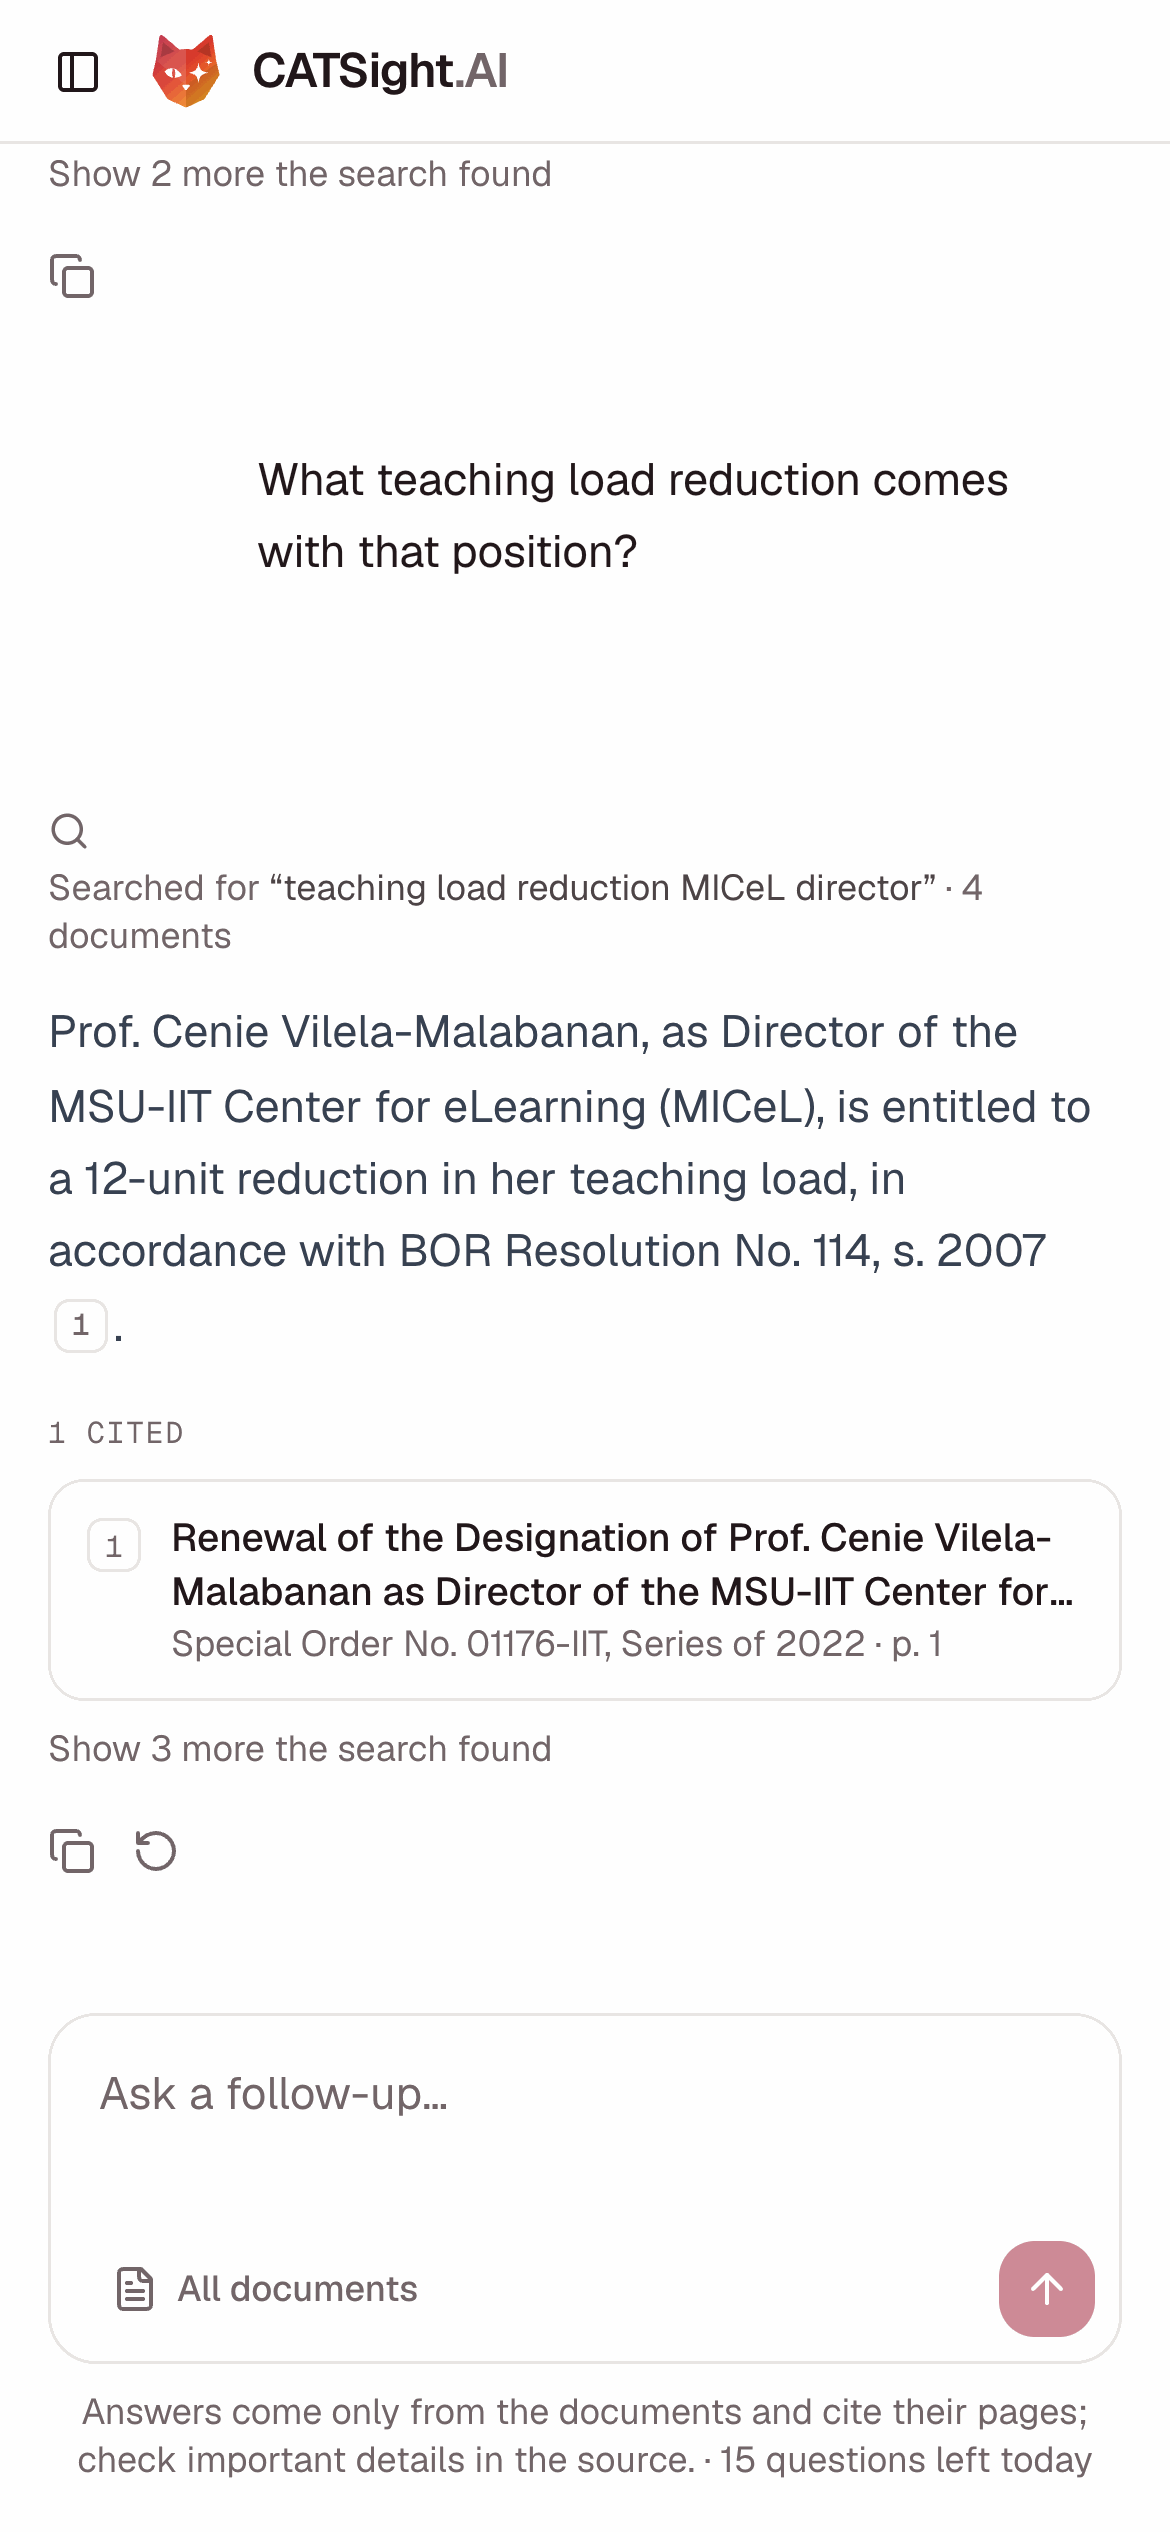
\includegraphics[height=9cm]{screenshots/mobile-chat}}\hspace{1.2cm}%
   \fbox{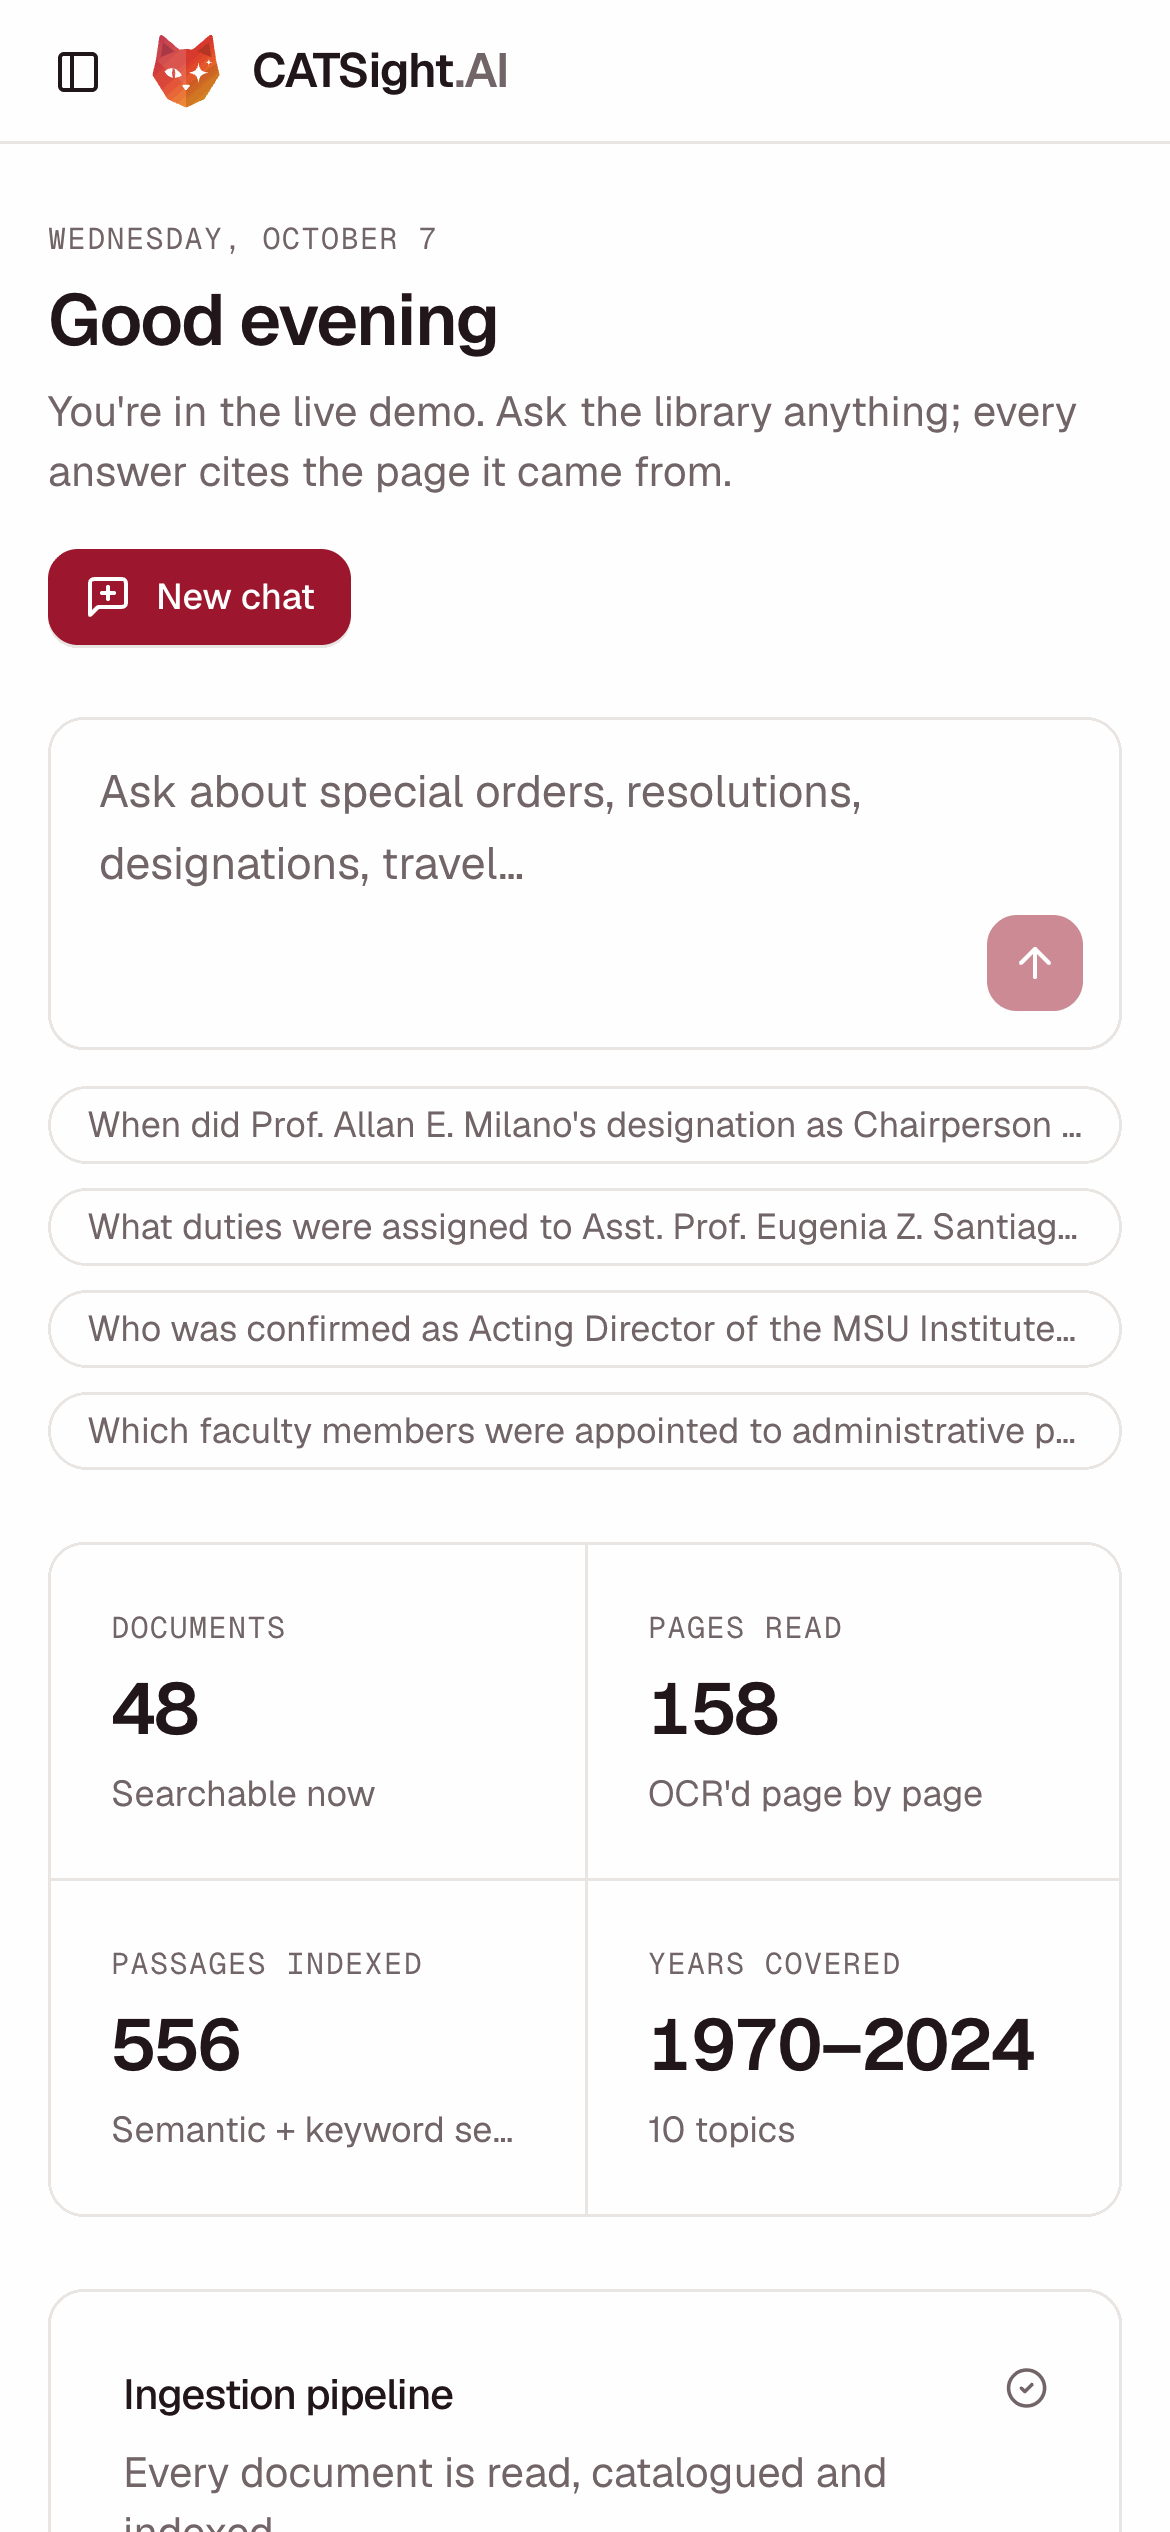
\includegraphics[height=9cm]{screenshots/mobile-dashboard}}}
  \caption{Chat and Dashboard on a Phone}\label{fig:mobile}
\end{figure}

\subsection{Environment and Resources}\label{sec:environment}

Table~\ref{tab:software} lists the software \cs{} is built with. The deployed system runs on a small on-premises server with an integrated GPU, which serves the OCR model; its containers, which cannot use the GPU, are allocated 10 CPU cores and 8~GB of memory. Development and the converter comparison of Section~\ref{sec:converter-comparison} used a laptop with an Apple M4~Pro processor and 24~GB of memory.

\begin{table}[htbp]
  \centering
  \caption{Software Used to Build \cs{}}\label{tab:software}
  \small
  \begin{tabularx}{\linewidth}{@{}>{\raggedright\arraybackslash}p{3.2cm}X@{}}
    \toprule
    \textbf{Layer} & \textbf{Software} \\
    \midrule
    Interface & React 18, TypeScript 5.6, Vite 6, Tailwind CSS 3.4, shadcn/ui, TanStack Query 5, react-pdf 9 (PDF.js) \\
    API & Python 3.11, Django 5.1, Django REST Framework 3.15, gunicorn 23, Server-Sent Events \\
    Document pipeline & Celery 5.5, Redis 7, pypdfium2 4.30, Marker 2.0 with Surya OCR 0.22, llama.cpp (build b11429), PyTorch (CPU) \\
    Retrieval and agent & LangChain 1.x, LangGraph 1.x with a PostgreSQL checkpointer \\
    Database & PostgreSQL 17 with pgvector and full-text search \\
    Models & Surya OCR 2, Qwen3-VL-30B-A3B-Instruct, BGE-M3, Qwen3-Reranker-8B (Table~\ref{tab:models}) through OpenRouter; Ollama for the local configuration \\
    Converters compared & Docling 2.134, MarkItDown 0.1.8 \\
    Deployment & Docker Compose, nginx, an outbound-only HTTPS tunnel \\
    \bottomrule
  \end{tabularx}
\end{table}

\section{Evaluation Procedure}\label{sec:evaluation-procedure}

The system is evaluated with the measures defined in Section~\ref{sec:evaluation-theory}.

\begin{enumerate}
  \item \textbf{Text extraction.} The four converters supported by \cs{} and two vision-model variants are run on a sample of seven documents (26 pages) chosen to cover pure scans, partial text layers, digital files, a watermark, tables, and a typewritten page from 1970. For each document, 8 to 11 facts (reference numbers, names, dates, amounts) were read from the page images, and a converter is credited with a fact when it appears in its output, ignoring case, spacing, punctuation, and leading zeros. Time per page is also recorded.
  \item \textbf{Retrieval accuracy.} A set of test questions, each with the documents that answer it, is run through \cs{}'s search and through the keyword search of IIT Docs; P@5, R@5, and MRR (Equations~\ref{eq:precision-recall} and~\ref{eq:mrr}) are compared. \TODO{Number of test questions and how the relevant documents were judged.}
  \item \textbf{Summary quality.} For a sample of documents, a person writes a reference summary without seeing the generated one; ROUGE-1, ROUGE-2, ROUGE-L, BLEU, and BERTScore (Equations~\ref{eq:rouge-n}--\ref{eq:bertscore}) compare each generated summary with its reference. \TODO{Number of documents and who wrote the references.}
  \item \textbf{Efficiency.} Search time is reported by the server for each search; time to first token and total response time are measured for chat answers; ingestion time is measured per page.
  \item \textbf{Usability.} Participants complete tasks with the existing system and with \cs{} and then answer the SUS questionnaire (Equation~\ref{eq:sus}) for each.
\end{enumerate}

\chapter{Design and Implementation Issue}\label{ch:design}

This chapter discusses the design and implementation of the major data structures and algorithms used in the software. It includes a discussion on the major issues and problems encountered, and the corresponding solutions and alternatives employed by the proponents. Parts of the design tools in the Technical Manual may be lifted as figures in this chapter.

This chapter discusses the design and implementation of the

\chapter{Results and Observations}\label{ch:results}

This chapter reports the results of the evaluation described in Section~\ref{sec:evaluation-procedure}. Because the system was rebuilt after the defense (Section~\ref{sec:scope}), each section states which version a result was measured on: the text-extraction comparison, the processing of the library, and the search and chat observations come from the rebuilt system in October 2026; the usability scores come from the evaluation of the defended prototype.

\section{Text Extraction}\label{sec:converter-comparison}

Table~\ref{tab:converters} and Figure~\ref{fig:converters} compare six ways of turning the seven sample documents (26 pages, 67 facts; Section~\ref{sec:evaluation-procedure}) into text. Four of the documents are pure scans or carry almost no text layer (36 facts); the other three carry a text layer produced by the repositories' own OCR.

\begin{table}[htbp]
  \centering
  \caption{Facts Recovered and Speed of Six Text-Extraction Setups}\label{tab:converters}
  \small
  \begin{tabularx}{\linewidth}{@{}>{\raggedright\arraybackslash}p{3.3cm}ccc>{\raggedright\arraybackslash}X@{}}
    \toprule
    \textbf{Setup} & \makecell{\textbf{All facts}\\(67)} & \makecell{\textbf{Scanned}\\(36)} & \makecell{\textbf{Seconds}\\\textbf{per page}} & \textbf{Observation} \\
    \midrule
    MarkItDown (text layer) & 27 (40\%) & 0\% & 0.01 & Nothing from scanned pages; repeats the repositories' OCR errors \\
    Docling (standard OCR) & 45 (67\%) & 56\% & 3.1 & Missed most of the watermarked BOR resolutions and the typewritten page \\
    Docling with Qwen3-VL & 64 (96\%) & 100\% & 6.4 & Shortened the surname ``Vilela-Malabanan'' \\
    Qwen3-VL on page images & 63 (94\%) & 97\% & 4.8 & Shortened the same surname; omitted three dates of issue \\
    Marker 2 (Surya OCR 2) & 58 (87\%) & 83\% & 13.8 & Exact names and dates; missed signatory names crossed by signatures and watermark-covered typewriting \\
    Marker 2 with Qwen3-VL & 61 (91\%) & 86\% & 22.2 & Exact names and dates, plus three signatory names; eight handwriting requests failed and kept Marker's text \\
    \bottomrule
  \end{tabularx}
  \par\smallskip
  \parbox{\linewidth}{\footnotesize\singlespacing\emph{Note.} Local models ran on a laptop GPU (Apple M4~Pro); Qwen3-VL-30B-A3B-Instruct ran through OpenRouter. Marker's time excludes the first document, which includes loading its models.}
\end{table}

\begin{figure}[htbp]
  \centering
  % Facts recovered by each converter on the seven-document sample (Table~\ref{tab:converters}).
\begin{tikzpicture}
  \begin{axis}[
      width=\linewidth, height=6.4cm,
      ybar, bar width=0.34cm, ymin=0, ymax=105, enlarge x limits=0.09,
      symbolic x coords={MarkItDown,Docling,Docling+VL,Qwen3-VL,Marker,Marker+VL},
      xtick=data, ylabel={Facts recovered (\%)},
      legend style={at={(0.02,0.98)}, anchor=north west, draw=none, font=\scriptsize, fill=none},
      legend cell align=left,
      nodes near coords, nodes near coords style={font=\tiny, text=ink},
      tick label style={font=\scriptsize}, label style={font=\footnotesize},
      axis lines*=left, ymajorgrids, grid style={line, densely dotted}]
    \addplot[fill=ink!65, draw=ink] coordinates {(MarkItDown,40) (Docling,67) (Docling+VL,96) (Qwen3-VL,94) (Marker,87) (Marker+VL,91)};
    \addplot[fill=maroon!75, draw=maroon] coordinates {(MarkItDown,0) (Docling,56) (Docling+VL,100) (Qwen3-VL,97) (Marker,83) (Marker+VL,86)};
    \legend{All seven documents, Four scanned documents}
  \end{axis}
\end{tikzpicture}

  \caption{Share of Facts Recovered by Each Text-Extraction Setup}\label{fig:converters}
\end{figure}

Three observations follow. First, the repositories' text layers are not enough: MarkItDown, which reads only those layers, recovered nothing from the scanned pages, so a system that indexes text layers alone cannot find a third of the corpus. Second, sending whole pages to a general vision-language model recovered the most facts, but its errors are of a dangerous kind: in both setups that did so, the model silently shortened an unusual surname, and when given page images directly it also skipped the date printed above the reference number. Such errors are plausible enough to go unnoticed, and they propagate into the catalogue; the summary of the affected special order, generated from that text, repeated the shortened name. Third, Marker's Surya OCR 2, a model trained only to transcribe, copied names, numbers, and dates exactly; its misses were text physically obscured by signatures and by the watermark on the 1970 resolution. Marker's LLM mode, in which Qwen3-VL corrects only the hard regions, recovered three more facts than Marker alone---signatory names partly covered by signatures---while keeping its exact names and dates. Eight of its requests on handwriting regions failed because the model repeated blank lines until its reply was cut off; Marker then kept Surya's own text for those regions, so a failed request costs only the improvement, never the text. \cs{} therefore uses Marker with its LLM mode: it gives up a few points of recall compared with the whole-page vision setups in exchange for transcriptions that do not silently alter names, numbers, or dates, which are what users search for.

Marker was also the slowest setup: about 14 seconds per page on a laptop GPU, 22 seconds with its LLM mode, and about two minutes per page on the laptop's CPU alone. This is acceptable for building a library, which happens once per document, but it is the main reason to run the OCR model on a GPU (Section~\ref{sec:issue-ocr-server}, Table~\ref{tab:gpu}).

\section{Processing of the Library}\label{sec:processing-results}

The deployed system processed all 48 documents with Marker~2---Surya OCR~2 with Qwen3-VL in LLM mode---and catalogued and indexed them with the open-weight models of Table~\ref{tab:models}. The library holds 158 pages split into 556 passages, issued between 1970 and 2024. Eleven documents failed during a brief restart of the OCR service and were resumed from the extracting stage without further intervention, as designed (Section~\ref{sec:issue-tasks}); none failed otherwise. Extraction dominated the processing time: with six pages read at once, the server extracted the last 132 pages in 94 minutes, about 43 seconds per page including Marker's LLM mode. Cataloguing took a median of 8.5 seconds per document and indexing 2.2 seconds. Each document received one to three of the 13 tags; Figure~\ref{fig:library-charts} shows how the documents are distributed across decades and tags.

\begin{figure}[htbp]
  \centering
  % The deployed library (48 documents) after reprocessing with Marker 2 and the open models, 7 October 2026.
\begin{tikzpicture}
  \begin{axis}[
      name=decades, width=6.4cm, height=6.2cm,
      ybar, bar width=0.55cm, ymin=0, ymax=30, enlarge x limits=0.15,
      symbolic x coords={1970s,1980s,2000s,2010s,2020s}, xtick=data,
      ylabel={Documents}, title={\footnotesize (a) By decade of issuance},
      nodes near coords, nodes near coords style={font=\scriptsize},
      tick label style={font=\scriptsize}, label style={font=\footnotesize},
      axis lines*=left, ymajorgrids, grid style={line, densely dotted},
      nodes near coords style={font=\scriptsize, text=ink}]
    \addplot[fill=maroon!75, draw=maroon] coordinates {(1970s,4) (1980s,1) (2000s,6) (2010s,25) (2020s,12)};
  \end{axis}
  \begin{axis}[
      at={($(decades.east)+(2.9cm,0)$)}, anchor=west, width=7.0cm, height=6.2cm,
      xbar, bar width=0.3cm, xmin=0, xmax=30, enlarge y limits=0.06,
      symbolic y coords={Memorandum,Academic Calendar,Suspension,Charter Day,Policy,Incentive,Travel Order,Other,Finance,Designation,Board Resolution,Special Order},
      ytick=data, xlabel={Documents}, title={\footnotesize (b) By tag (a document has 1--3 tags)},
      nodes near coords, nodes near coords style={font=\scriptsize},
      tick label style={font=\scriptsize}, label style={font=\footnotesize},
      axis lines*=left, xmajorgrids, grid style={line, densely dotted},
      nodes near coords style={font=\scriptsize, text=ink}]
    \addplot[fill=ink!65, draw=ink] coordinates {(1,Memorandum) (2,Academic Calendar) (3,Suspension) (5,Charter Day) (6,Policy) (9,Incentive) (11,Travel Order) (17,Other) (17,Finance) (21,Designation) (23,Board Resolution) (25,Special Order)};
  \end{axis}
\end{tikzpicture}

  \caption{The Library by Decade of Issuance and by Tag}\label{fig:library-charts}
\end{figure}

\section{Retrieval}\label{sec:retrieval-results}

Figures~\ref{fig:search-identifier} and~\ref{fig:search-semantic} show the two kinds of matching at work. A search for ``SO 1592'' (Figure~\ref{fig:search-identifier}) finds Special Order No.~01592-IIT although the query omits the leading zero and the word ``Special Order'': the keyword search matches the normalized number, and the passage is labelled an exact match. A search for ``scholarship stipend for engineering technology students'' (Figure~\ref{fig:search-semantic}) finds the 2003 resolution on grants-in-aid, whose text speaks of ``Grants-in-Aid'' and ``School of Engineering Technology'' rather than ``scholarship stipend'': here the semantic search contributes. When the query is a question, the search page also writes a short cited answer above the results (Figure~\ref{fig:search-answer}).

\screenshot{search-identifier}{Search by Reference Number: ``SO 1592'' Finds Special Order No. 01592-IIT}
\screenshot{search-semantic}{Search by Meaning: a Paraphrased Query Finds the Grants-in-Aid Resolution}
\screenshot{search-answer}{A Question in the Search Page, with a Short Cited Answer}

Table~\ref{tab:retrieval} compares the retrieval accuracy of \cs{} with the keyword search of IIT Docs.

\begin{table}[htbp]
  \centering
  \caption{Retrieval Accuracy}\label{tab:retrieval}
  \begin{tabular}{@{}lccc@{}}
    \toprule
    \textbf{System} & \textbf{P@5} & \textbf{R@5} & \textbf{MRR} \\
    \midrule
    IIT Docs (keyword search) & \TODO{} & \TODO{} & \TODO{} \\
    \cs{} (hybrid search) & \TODO{} & \TODO{} & \TODO{} \\
    \bottomrule
  \end{tabular}
\end{table}

\section{Chat}\label{sec:chat-observations}

Asked who was designated Director of the MSU-IIT Center for eLearning in 2022 (Figure~\ref{fig:chat-answer} in Chapter~\ref{ch:methodology}), the chat searched, named the faculty member and the effectivity date with a citation to Special Order No.~01176-IIT, and noted that the order does not state a fixed term. The follow-up in Figure~\ref{fig:chat-follow-up} refers only to ``that position''; the assistant searched for the teaching-load reduction of the MICeL director and answered with the 12-unit reduction granted under BOR Resolution No.~114, s.~2007, citing the order. In a chat limited to the 2003 grants-in-aid resolution (Figure~\ref{fig:chat-scoped}), it read the whole resolution and answered that the new maximum monthly stipend of a full grantee is PhP 1,200.00, broken down into meals and lodging. A question in Filipino was answered in Filipino from an English resolution, with a citation (Figure~\ref{fig:chat-filipino}).

These answers came after three fixes described in Chapter~\ref{ch:design}. In the first run on the rebuilt system, the same follow-up was answered without a search---the documents ``do not specify'' the reduction---the scoped question was answered with PhP 800, the old maximum quoted in the resolution's rationale, and most answers carried no citation numbers (Sections~\ref{sec:issue-followup}--\ref{sec:issue-citations}). Neither wrong answer invented a fact, but both would have misled a reader who did not open the source. After the fixes, all eight answers in a check of eight questions carried citations, and both questions were answered correctly.

\screenshot{chat-follow-up}{A Follow-Up Question Answered from the Conversation}
\screenshot{chat-scoped}{A Chat Limited to One Document}
\screenshot{chat-filipino}{A Question in Filipino Answered in Filipino}

\section{Summary Quality}\label{sec:summary-results}

Table~\ref{tab:summary-metrics} reports the agreement of the generated summaries with the human-written references (Section~\ref{sec:summary-metrics}).

\begin{table}[htbp]
  \centering
  \caption{Summary Quality against Human-Written References}\label{tab:summary-metrics}
  \begin{tabular}{@{}lccccc@{}}
    \toprule
    & \textbf{ROUGE-1} & \textbf{ROUGE-2} & \textbf{ROUGE-L} & \textbf{BLEU} & \textbf{BERTScore F$_1$} \\
    \midrule
    \cs{} & \TODO{} & \TODO{} & \TODO{} & \TODO{} & \TODO{} \\
    \bottomrule
  \end{tabular}
\end{table}

\section{Efficiency}\label{sec:efficiency-results}

Table~\ref{tab:efficiency} reports response times measured on the deployed system as a guest, over the public internet, with five searches and five chat questions. A search takes about 3.3 seconds, which includes embedding the query, running both searches, and reranking, all with models reached over the internet. A chat answer streams: the search finishes after about 1.3 seconds, the first words of the answer appear after a median of 9.1 seconds, and the answer is complete after about 14 seconds. The hosted models' response times vary with load: earlier runs on the same day had medians as low as 5.1 seconds to the first word and 8.5 seconds to a complete answer. Building the library is slower, at about 43 seconds per page (Section~\ref{sec:processing-results}), but it happens once per document.

\begin{table}[htbp]
  \centering
  \caption{Response Times of the Deployed System}\label{tab:efficiency}
  \begin{tabular}{@{}lcc@{}}
    \toprule
    \textbf{Measure} & \textbf{Median} & \textbf{Range} \\
    \midrule
    Search (5 queries) & 3.3 s & 2.3--5.3 s \\
    Chat: search completed (5 questions) & 1.3 s & 1.1--2.4 s \\
    Chat: first word of the answer & 9.1 s & 6.4--10.0 s \\
    Chat: complete answer & 13.6 s & 11.0--15.0 s \\
    Extraction of a page (132 pages) & \multicolumn{2}{c}{43 s on average} \\
    \bottomrule
  \end{tabular}
\end{table}

\section{Usability}\label{sec:usability-results}

In the usability evaluation of the defended prototype, participants rated \cs{} at an average of 77.17 on the System Usability Scale, against 50.33 for the existing keyword-based system. On the adjective scale of \citet{bangor2009}, a score in the high 70s corresponds to ``good'' usability and a score near 50 to ``OK'' or marginal usability, below the commonly cited average of 68. The difference of almost 27 points reflects what the participants could do with \cs{} that the existing system did not allow: ask in their own words, search scanned documents, and see the source of an answer. \TODO{Number of participants and their roles (students, faculty, staff) from the defended evaluation.} The interface was redesigned in the rebuilt system, so the study should be repeated with it (Chapter~\ref{ch:conclusion}).

\chapter{Conclusion and Recommendations}\label{ch:conclusion}


\appendix
\renewcommand{\cftchappresnum}{Appendix~}
\titleformat{\chapter}[block]{\normalfont\large\bfseries}{Appendix \thechapter}{0.5em}{}
\chapter{Bibliography}\label{app:bibliography}
\begingroup
\renewcommand{\chapter}[2]{}% the bibliography's own heading is replaced by the appendix title
\singlespacing
\nocite{*}
\bibliographystyle{apalike}
\bibliography{references}
\endgroup
\chapter{Personal Vitae}\label{app:vitae}

\section*{Arellano, Carlo P.}
\TODO{Vitae from the defended manuscript (Appendix B): photo, contact, education, skills.}

\section*{Carnaje, Michael James M.}
\TODO{Vitae from the defended manuscript (Appendix B): photo, contact, education, skills.}

\section*{Lavesores, Fulgent Kvasir E.}
\TODO{Vitae from the defended manuscript (Appendix B): photo, contact, education, skills.}


\end{document}
